\documentclass{article}

\usepackage{latexsym}
\usepackage{fancyhdr}
\usepackage{algorithm}
\usepackage[noend]{algpseudocode}
\usepackage{amsmath}
\usepackage{amsthm}
\usepackage{amssymb}
\usepackage{mathtools}
\usepackage{amsthm}
\usepackage{hyperref}
\usepackage{listings}
\usepackage{scrextend}
\usepackage{dirtytalk}
% \usepackage[demo]{graphicx}
\usepackage{caption}
\usepackage{subcaption}
\usepackage{pdfpages}
\usepackage[shortlabels]{enumitem}
\usepackage[margin=1.2in]{geometry}
\lhead{Charles Pehlivanian}
\rhead{Consecutive Partitions For Power Score Functions}
\cfoot{\thepage}
\pagestyle{fancy}

\hypersetup{colorlinks=true, urlcolor=blue}

\newtheorem{thm}{Theorem}
\newtheorem{definition}{Definition}
\newtheorem{lemma}{Lemma}
\newtheorem{sublemma}{Lemma}[lemma]
\newtheorem{corollary}{Corollary}
\newtheorem{prop}{Proposition}

\newtheoremstyle{case}{}{}{}{}{}{:}{ }{}
\theoremstyle{case}
\newtheorem{case}{Case}

\DeclareMathOperator*{\argmax}{argmax} % thin space, limits underneath in displays
\DeclareMathOperator*{\argmin}{argmin} % thin space, limits underneath in displays
\newcommand{\stirlingii}{\genfrac{\{}{\}}{0pt}{}}

\newenvironment{example}[1]{\par\noindent\underline{Example:}\space#1}{}

\newenvironment{claim}[1]{\par\noindent\underline{Claim:}\space#1}{}
\newenvironment{claimproof}[1]{\par\noindent\underline{Proof:}\space#1}{\hfill $\blacksquare$}

\makeatletter
\def\BState{\State\hskip-\ALG@thistlm}
\makeatother

\begin{document}
\sloppy

\begin{abstract}
	A number of combinatorial optimization problems involve maximization or minimization of the sum of an $\mathbb{R}$-valued set function $F$ over subsets of a partitions of a base set $S$. A common case occurs when the base set is finite $\left\lbrace 1, \dots, n\right\rbrace$, and each element is associated with attributes $x_i$, $y_i$ contributing to a score -the inner step of many iterative algorithms - gradient boosting, unsupervized clustering, image compression, network detection - rely on maximization of a power function $F(x,y) = x^{\alpha}y^{-\beta}$ over a suitably labeled base set. It is well-known that the maximization problem for submodular $F$ is NP-hard. We give a set of conditions on $F$ so that exact results can be obtained by constrained maximization over a much smaller set of partitions, for any attribute labeling. We also address a gap in the existing literature by clearly distinguishing strict and weak size $T$ partitions and giving sufficient conditions for the existence of strongly optimal partitions. The results allow for $\mathcal{O}\left( n^{T-1}\right)$ maximization cost, although it is shown that with unbounded memory the problem is no worse than $\mathcal{O}\left(n^2\right)$. Finally many of the linear time subset scan algorithms (LTSS) in a spatial scan statistics setting can be obtained with this approach.
\end{abstract}

\section{Preliminaries}
Let $n \in \mathbb{N}$ be positive and set $\mathcal{V} = \{1, \dots, n\}$. Let $X = \left\lbrace x_1, \dots, x_n\right\rbrace$, $Y = \left\lbrace y_1, \dots, y_n\right\rbrace$ be real sequences with $y_i > 0$, for all $i$. The tuple $\left(x_i, y_i\right)$ is called a $\textit{record}$ and denoted by $R_i$. Denote by $\mathcal{D} = \mathcal{D}_{X,Y}$ the set of records $\left\lbrace \left( x_i, y_i\right) \right\rbrace$ associated with the sequences $X$, $Y$. The sequence of records is assumed to have an order induced by a priority function on the sequences $X$, $Y$.

\begin{definition}
A priority function is a function $G\colon \mathbb{R} \times \mathbb{R}^{+} \to \mathbb{R}$ that induces an ordering on the tuples $R_i = \left(x_i, y_i\right)$. We refer to $G(x,y) = \frac{x^{\tau}}{y}$ as a power priority function, and the case $\tau = 1$ as the standard priority function. The ordering induced on the sequences $X$, $Y$ induced by $G$ is denoted by $R_{(1)}, R_{(2)}, \dots R_{(n)}$, representing, in order, the highest priority record, next highest, etc., with $x_{\left( i\right)}$, $y_{\left( i\right)}$ the components of the record $R_{\left( i\right)}$.
\end{definition}

No continuity or smoothness assumptions are made on $G$. In fact, we will focus attention on the standard priorty function as will be evident from Proposition 1 below, and unless otherwise stated we assume that the elements of the records $R_1, \dots, R_n$ are ordered by the standard priority.

A partition $\mathcal{P}$ of size $t$ of $\mathcal{V}$ is specified by a set of subsets $\mathcal{P} = \{ P_1, \dots, P_t \}$, $P_i \subseteq N$, $i = 1, \dots, t$, such that $P_1 \cup \dots \cup P_t = \{1, \dots, n\}$, with the $P_i$'s pairwise disjoint. Each subset $S \subseteq \mathcal{V}$ can be identified with a point $p_S = (\sum_{i \in S} x_i, \sum_{i \in S}y_i) \in \mathbf{R}^2$, called the polytope point of $P$, with $p_{\emptyset} = (0,0)$ by convention. In this way $\mathcal{P}$ is associated with a pointset in $\mathbf{R}^2$ through $X$, $Y$.

The elements $x_i$ and $y_i$ can be thought of as contributing to a scalar score for the record $R_i$. Often $x_i$ is a realization or exceedence over expectations and $y_i$ is a baseline expectation or deviation measure. This is the approach taken in online spatial event detection methods in the context of spatial scan statitistics and real-time detection of emerging events. In this setting, detection of clusters corresponding to outbreaks of disease, suspicious activity, areas of increased brain activity from fMRI imaging, etc., is isolated from spatial time series data by maxiizing a likelihood ratio statistic over subsets of the data, in a constrained or unconstrained optimization (see $\cite{article6}$ $\cite{article8}$, $\cite{article9}$, e.g.). In the usual setting the $x_i$ correspond to occurences while the $y_i$ represent baselines or expectations and regions of maximal occurence or density must further be determined as significant or not. The objective function to be maximized is usually called the $\textit{score}$ function, the maximization over all subsets of the spatial data represents an unconstrained combinatorial optimiziation problem. The unconstrained problem is often computationally infeasible (of exponential order), but linear-time exact algorithms have been developed under the name LTSS (Linear Time Subset Scan). We give an alternate geometric derivation of these results as a corollary of the classification of extreme points for an associated polytope in $\mathbf{R}^2$ (Proposition 1). In addition, our main result is applicable to cluster detection problems in the Gaussian case, see below. The notion of a score function is formalized below.

\begin{definition}
A score function is a continuous $F(x, y)\colon \mathbb{R} \times \mathbb{R}^{+} \to \mathbb{R}$, strictly increasing in $x$ and strictly decreasing in $y$, with $F\left( 0,0\right) = 0$. If F is of the form $F(x,y) = x^\alpha y^{-\beta}$ for some $\alpha, \beta > 0$, then F is a rational score function. For any one of $\alpha$, $\beta$ noninteger we assume that $F$ takes real values, i.e. that $X \subseteq \mathbf{R}^+$.
\end{definition}

Several additional properties have been associated with score functions, namely quasi-convexity, componentwise convexity, or a marginal contribution constraint $\frac{x}{y} \frac{\partial F}{\partial x} + \frac{\partial F}{\partial y} \geq 0$ related to submodularity. We do not assume smoothness beyond continuity, nor (quasi)convexity, unless explicitly stated.

A score function $F$ gives rise to a function (also denoted by $F$ when the context is clear) $F \colon 2^N \rightarrow \mathbb{R}$ by summation over individual subset elements $F(S) = F(\sum_{i \in S} x_i, \sum_{i \in S} y_i)$, for $S \subseteq N$. Associating $S \subseteq N$ with its $X$, $Y$ attributes as in $X_S = \left\lbrace x_i \colon i \in S\right\rbrace$, $Y_S = \left\lbrace y_i \colon i \in S\right\rbrace$ allows us to write $F(S) = F(X_S, Y_S) = F(\sum_{x \in X_S}x, \sum_{y \in Y_S}y)$, etc.

Now fix a partition $\mathcal{P} = \left\lbrace P_1, \dots, P_t\right\rbrace$ of size $t$ of $N$. We are interested in maximal partitions for $F$, i.e., solutions to the program
\begin{align} \label{eq0}
\mathcal{P}^{*} = \argmax_{\substack{\mathcal{P} = \left\lbrace P_1 \dots, P_t\right\rbrace}} {\sum\limits_{j=1}^{T}F\left( X_j, Y_j\right)} = \argmax_{\substack{\mathcal{P} = \left\lbrace P_1, \dots, P_t\right\rbrace}} {\sum\limits_{j=1}^{T}F( \sum_{i \in P_j}x_i, \sum_{i \in P_j}y_i)}
\end{align}
which for a power score function becomes
\begin{align} \label{eq1}
\mathcal{P} = \argmax_{\substack{\mathcal{P} = \left\lbrace \pi_1 \dots, \pi_T\right\rbrace}}\sum_{j=1}^{T}\frac{(\sum_{i \in P_j}x_i)^\alpha}{(\sum_{i \in P_j}y_i)^\beta}
\end{align}

\vspace{4pt}

For example, given a set of quadratic polynomials $p_i(x) = \frac{1}{2}h_ix^2 + g_ix + c_i$, with $h_i >0$ for all $i$, the minimum values are $\frac{-g_i^2}{2h_i}$. Associating each polynomial with the record $(-g_i, h_i)$, the standard priority function orders them by the x-coordinate of the vertex, $\frac{-g_i}{h_i}$. The solution to $\ref{eq1}$ for $\alpha = 2$, $\beta = 1$ finds the x-values $\left\lbrace x_1, \dots, x_t\right\rbrace$ that minimizes the sum $\sum_{j=1}^t \sum_{i \in P_j} p_i\left( x_j\right) = \sum_{j=1}^t p_{S_j}$, where $p_{S_j}$ is the quadratic $\sum_{i \in P_j} p_j$, or equivalently, the partition of $\mathcal{V}$ for which subset sums of the polynomials achieves the minimal value.

It is well-known that for $F$ submodular, the maximization program in $\ref{eq1}$ above is NP-hard (while the minimization problem can be solved in polynomial time) $\cite{article7}$, $\cite{article10}$. For maximization of non-monotone submodular objectives, any polynomial time algorithm is only guaranteed to have a lower bound of $\frac{1}{2}$ from optimality, i.e., $F(S) \geq \frac{1}{2}F(S^{*})$, where $S^*$ is the argmax. A complete search of the space of size $T$ partitions is only feasible for small $N$, well under the typical size of most modern training sets. It will be necessary to constrain our attention to a smaller set of partitions.

\begin{definition}
A subset $S \subseteq N$ is consecutive if it is of the form $\left\lbrace j, j+1, \dots k\right\rbrace$, for $1 \leq j \leq k \leq n$, or it is the empty set. A consecutive subset $P \subseteq \mathcal{V}$ is nonsplitting if both $P$, $\mathcal{V}  \backslash P$ are consecutive. Otherwise, it is splitting. Define
\begin{align*}
\mathcal{T} &= \mathcal{T}_n = \{ P \subseteq \mathcal{V} : P \textrm{ is consecutive} \}\\
\mathcal{S} &= \mathcal{S}_n = \{ P \subseteq \mathcal{V} : P \textrm{ is consecutive, splitting} \} \\
\mathcal{U} &= \mathcal{U}_n = \{ P \subseteq \mathcal{V} : P \textrm{ is consecutive, non-splitting}\} \\
\underline{\mathcal{U}} &= \underline{\mathcal{U}}_n = \mathcal{U}_n \setminus \left\lbrace p_{\emptyset}, p_{\mathcal{V}}\right\rbrace
\end{align*}
\end{definition}


A special case of a consecutive subset occurs when $P$ is a singleton $\left\lbrace j\right\rbrace$; the pair $P$, $\mathcal{V}\setminus P$ will be called a $\textit{singleton splitting}$ or $\textit{non splitting}$ pair, depending on whether $\mathcal{V}\setminus P$ is consecutive. The set of singleton splitting subsets and their complements in $\mathcal{V}$ is denoted by 
\begin{align*}
\mathcal{\underline{S}} = \underline{\mathcal{S}_n}  = \{ P \subseteq \mathcal{V} \colon (P, \mathcal{V} \setminus P) \textrm{ form a singleton splitting pair}\}\subseteq \mathcal{S}_n
\end{align*}

For any partition $\mathcal{P} = \left\lbrace S_1, \dots, S_t\right\rbrace$ denote by $\Pi$ the mapping taking $\mathcal{P}$ to the set $\left\lbrace \left\lbrace p_{S_1}\right\rbrace, \dots, \left\lbrace p_{S_t}\right\rbrace \right\rbrace$ in $\mathbf{R}^2$, so that $\Pi\left( \mathcal{S}\right) \subseteq \Pi\left( \mathcal{T}\right)$, $\Pi\left( \mathcal{U}\right) \subseteq \Pi\left( \mathcal{T}\right)$, $\Pi\left( \mathcal{\underline{S}}\right) \subseteq \Pi\left( \mathcal{S}\right) \cup \Pi\left( \mathcal{U}\right)$, etc.

% \begin{align*}
% \Pi\left( \mathcal{T}_n\right) &= \left\lbrace p_S \colon S \in \mathcal{T}_n\right\rbrace \\
% \Pi\left( \mathcal{S}_n\right) &= \left\lbrace p_S \colon S \in \mathcal{S}_n\right\rbrace \\
% \Pi\left( \mathcal{U}_n\right) &= \left\lbrace p_S \colon S \in \mathcal{U}_n\right\rbrace \\
% \Pi\left( \underline{\mathcal{S}}_n\right) &= \left\lbrace p_S \colon S \in \underline{\mathcal{S}}_n\right\rbrace \\
% \end{align*}

It is easy to see that $| \mathcal{U}_n | = 2n - 1$, $| \mathcal{S}_n | = \frac{(n-1)(n-2)}{2}$, with $| \mathcal{T}_n | = | \mathcal{U}_n | + | \mathcal{S}_n | = \frac{n(n+1)}{2}$, while $| \underline{\mathcal{S}}_n | = 2n - 2$. A search over consecutive non-splitting subsets can be performed in linear time, while over consecutive splitting subests the search time is quadratic in $n$.

\begin{definition}
A partition $\mathcal{P} = \left\lbrace P_1, \dots, P_T\right\rbrace$ of $N$ of size $t$ such that each $P_i$ is a consecutive subset is called a consecutive partition. If every subset of a consecutive partition is nonempty, then it is strongly consecutive, otherwise we allow a weakly consecutive partition to contain $s < t$ nonempty subsets.
\end{definition}

It is known (see $\cite{article1}$, $\cite{article2}$) that if $F$ is convex, or convex in all of its arguments, and $y_i > 0$, for all $i$, that a weakly consecutive partition exists that is maximal in the sense of $\ref{eq1}$ for the standard priority function. The authors allude to the possibility of empty partition subsets (giving rise to a weakly consecutive partition) as a kind of degenerate case that falls out of the regular line of reasoning. Unfortunately, even in the convex case we can only assure that the maximal partition has size $s \leq t$, and degeneracy is related to a common nondegenerate proprty in a polytope associated with the sequences $X$, $Y$ (see Section 2). 
Furthermore, the collapsing of size can be dramatic, as shown by the examples below.

On the other hand, set of partitions is greatly reduced by the requirement that $\mathcal{P}$ be strongly consecutive. The set of all partitions of $n$ is a Bell number, exponentially increasing with $n$ for any $t > 1$. The set of all size $t$ partitions which we denote by $\mathcal{P}_{n,t}$ is a Stirling number of the second kind $\stirlingii{n}{t}$. The $n$th Bell number $B_n$ is given by the identity
\[B_n = \sum_{k=0}^{n} \binom{n}{k} B_k\]
The Stirling numbers follow the recursion
\[S_{n+1,k} = \stirlingii{n+1}{k} = k\stirlingii{n}{k} + \stirlingii{n}{k-1}\]
and have asymptotic growth rate 
\[\stirlingii{n}{k} \sim \frac{k^n}{k!}\]

The set $\mathcal{T}_{n,t}$ of consecutive partiions of $\mathcal{V}$ of size $t$ has size $\binom{n-1}{t-1}$, which grows as $\mathcal{O}\left( n^{t-1}\right)$. So for $\left(n,t\right) = \left(20, 10\right)$, we have $\vert \mathcal{P}_{n,t}\vert \approx 5.9e12$, $\vert \mathcal{T}_{n,t}\vert = 92378$, while for $\left(n,t\right) = \left(30, 10\right)$, we have $\vert \mathcal{P}_{n,t}\vert \approx 1.73e22$, $\vert \mathcal{T}_{n,t}\vert = 10,015,005$.  Although the polynomial growth of $\mathcal{T}_{n,t}$ may not be attractive, we outline a dynamic programming approach which guarantees worst-case quadratic time, for any $t$, with memory requirements that grow as $\mathcal{O}\left( nt\right)$


\vspace{4pt}

\begin{example}
Let $X = \left\lbrace 8, 2, 9\right\rbrace$, $Y = \left\lbrace  8, 1, 3\right\rbrace$, $G$ the standard priority function and $F$ the power score function with $\gamma = 4$. It is clear that $F$ is componentwise convex and convex. There are 3 partitions of the set $\mathcal{V} = \left\lbrace 1,2,3 \right\rbrace$ and direct evaluation gives
\begin{verbatim}
      PARTITION: [[1, 2], [3]]
          SUBSET: [1, 2] SUBSET SCORE: 1111.1111
          SUBSET: [3] SUBSET SCORE: 2187.0
          PARTITION SCORE: 3298.1111
      PARTITION: [[1], [2, 3]]
          SUBSET: [1] SUBSET_SCORE: 512.0
          SUBSET: [2, 3] SUBSET SCORE: 3660.25
          PARTITION SCORE: 4172.25
      PARTITION: [[1, 3], [2]]
          SUBSET: [1, 3] SUBSET SCORE: 7592.8182
          SUBSET: [2] SUBSET SCORE: 16.0
          PARTITION SCORE: 7608.8182
      MAX PARTITION SCORE: 7608.8182, MAX_PARTITION: [[1, 3], [2]]
\end{verbatim}
In this case no strongly consecutive partition of size 2 exists as the optimal partition is nonconsecutive. A weakly consecutive partition of size $t = 1$ exists consisiting of the trivial partition of $\mathcal{V}$ with maximal score given by
\begin{verbatim}
      PARTITION: [[1, 2, 3]]
          SUBSET: [1, 2, 3] SUBSET SCORE: 10860.0833
          PARTITION SCORE: 10860.0833
      MAX PARTITION SCORE: 10860.0833, MAX_PARTITION: [[0, 1, 2]].
\end{verbatim}  
\end{example}

\begin{example}
Let 
\begin{align*}
X & = \left\lbrace 0.992819, 0.04904, 0.622353, 0.464107, 0.608956, 0.984192 \right\rbrace \\
Y & = \left\lbrace 0.935323, 0.02541, 0.279373, 0.205452, 0.24599, 0.315633 \right\rbrace,
\end{align*}
$G$ the standard priority and $\gamma = 4$. $\frac{X}{Y} \approx \left\lbrace 1.0614718, 1.9299488, 2.2276777, 2.2589559, 2.4755315, 3.118153 \right\rbrace$. $F$ is again convex, but the only maximal consecutive partition of weak size $t = 5$ is the trival size-1 partition. We have

\begin{verbatim}
    Maximal 5-partition
    PARTITION: [ 0 5 ][ 1 ][ 2 ][ 3 ][ 4 ]
    SUM OF SCORES: 13.5342629367

    Maximal 4-partition
    PARTITION: [ 0 4 5 ][ 1 ][ 2 ][ 3 ]
    SUM OF SCORES: 30.6365105858

    Maximal 3-partition
    PARTITION: [ 0 2 4 5 ][ 1 ][ 3 ]
    SUM OF SCORES: 59.8732051128

    Maximal 2-partition
    PARTITION: [ 0 2 3 4 5 ][ 1 ]
    SUM OF SCORES: 91.7825870559

    Maximal 1-partition
    PARTITION: [ 0 1 2 3 4 5 ]
    SUM OF SCORES: 95.5586821397
\end{verbatim}
In fact the trivial partition is the optimal partition of size $t \leq 5$, and there are no strongly consecutive maximal partitions for any $t \in \left\lbrace 2, 3, 4, 5\right\rbrace$.

\end{example}

In fact for any pair $\left( n, t\right)$ a maximally-degenerate collapsing specification in $X$, $Y$ exists for any convex score function that isn't subadditive. A search over the consecutive partitions of size $t$ at the top level is incomplete; it may be the case that the optimal partition is weakly consecutive, which says nothing about the optimizing partition of strict size $t$. There is no way to know whether the size $t$ strongly consecutive maximizing partition is globally optimal, and one must repeat the process for size $t-1, \dots$. 

\vspace{4pt}

We will first give general conditions which guarantee the existence of a strongly consecutive maximal partition, which can be easily checked for many specifications of $F$, including rational score functions, which can be completely classified. Furthermore, even in the weakly consecutive case, an interleaving property is shown allowing for a constrained search and a worst-case $O(N^2)$ exact algorithm $\textit{even in the weakly consecutive case}$. Applications are given in Section 3.

\section{Main Results}
We now state our main results. 

\begin{definition}
For any $\mathcal{P}$ a partition of $\mathcal{V}$, the partition polytope $\mathcal{C} \subseteq \mathbb{R}^2$ of $\mathcal{P}$ is defined by $\mathcal{C} = convhull \left\lbrace p_S : S \in \mathcal{P}\right\rbrace$. The constrained partition polytope of $\mathcal{P}$ is defined by $\underline{\mathcal{C}} = convhull \left\lbrace p_S : S \in \mathcal{P}, S \neq \emptyset , S \neq \mathcal{V}\right\rbrace$
\end{definition}

A subset of records ordered by the standard priority in $\mathcal{D}$ is consecutive if it is of the type $\left\lbrace R_{(j)}, R_{(j+1)}, \dots, R_{(k)}\right\rbrace$, for $1 \leq j \leq k \leq n$ with the ordering from $G$. For the following Proposition, the importance of the standard priority function is established. An elementary technical lemma is needed.

\begin{lemma}
For $\frac{x_1}{y_1} \leq \frac{x_2}{y_2} \leq \dots \leq \frac{x_k}{y_k}$, $y_i > 0$, for all $i$,
\begin{align*}
\frac{x_1}{y_1} \leq \frac{x_1 + \dots + x_k}{y_1 + \dots + y_k} \leq \frac{x_k}{y_k},
\end{align*}
with equality if and only if $\frac{x_1}{y_1} = \dots = \frac{x_n}{y_n}$.
\end{lemma}
\begin{proof}
For $k=2$,
\begin{align*}
\frac{x_1+x_2}{y_1+y_2} - \frac{x_1}{y_1} = \frac{x_1y_2 - x_2y_1}{y_1\left( y_1 + y_2\right)} &\geq 0 \\
\frac{x_1 + x_2}{y_1 + y_2} - \frac{x_2}{y_2} = \frac{x_1y_2 - x_2y_1}{y_2\left( y_1 + y_2\right)} &\leq 0.
\end{align*}
For $k > 2$, two applications of the above case gives
\[
\frac{x_1}{y_1} \leq \frac{\sum_1^{k-1} x_i}{\sum_1^{k-1} y_i} \leq \frac{\sum_1^k x_k}{\sum_1^k y_i} \leq \frac{x_k}{y_k}. 
\]
If $\frac{x_1}{y_1} = \frac{x_n}{y_n}$, then the ordering in the assumptions implies all ratios are equal. 
\end{proof}

\begin{prop} \label{prop0}
Let $\mathcal{D}$ be a set of records with standard priorty function $G$. Define $\mathcal{E} = \left\lbrace \textit{extreme points of } \mathcal{C}\right\rbrace$, $\underline{\mathcal{E}} = \left\lbrace \textit{extreme points of } \underline{\mathcal{C}}\right\rbrace$. Then
\begin{enumerate}[(i)]
	\item $\mathcal{E} = \Pi\left( \mathcal{U}\right)$
	\item $\Pi\left( \mathcal{\underline{U}}\right) \subseteq \underline{\mathcal{E}} \subseteq \Pi\left( \mathcal{\underline{U}}\right) \cup \Pi\left( \mathcal{\underline{S}}\right)$
\end{enumerate}
\end{prop}

In particular $\underline{\mathcal{E}}$ contains most consecutive nonsplitting subsets, may contain consecutive splitting subsets, (but only singletons), and possibly nonconsecutive elements associated with a singleton splitting pair, while $\mathcal{E}$ contains only consecutive nonsplitting elements.
\begin{proof}
Let $p ^* = (x^*, y^*) \in \mathcal{E}$. Then there is an affine $a\left(x,y\right) = Ax + By + C$ satisfying $a(x^*, y^*) = 0$, $a(x,y) < 0$ for all $(x,y) \in \mathcal{C} \setminus p^*$.  We have
\begin{align}
Ax^* + By^* = \min_{(x,y) \in \mathcal{C}} Ax + By = \min_{S \subseteq \mathcal{V}} \sum_{i \in S} (Ax_i + By_i).
\end{align}
The set $S^* = \{ i \in \mathcal{V}: Ax_i + By_i \leq 0 \}$ minimizes the last expression. We will show that $S^*, \mathcal{V}\setminus S^*$ are both consecutive. If $A = 0$ then necessarily $B \neq 0$. If $B > 0$ then $S^* =\left\lbrace i \in \mathcal{V} \colon y_i \leq 0 \right\rbrace = \emptyset$, otherwise $S^* = \left\lbrace i \in \mathcal{V}  \colon y_i \geq 0 \right\rbrace = \mathcal{V}$, in either case both $S^*$, $\mathcal{V}\setminus S^*$ are consecutive. If $ A \neq 0$ then $S^* = \left\lbrace i \in \mathcal{V} \colon \frac{x_i}{y_i} \leq -\frac{B}{A} \right\rbrace$ or $S^* = \left\lbrace i \in \mathcal{V} \colon \frac{x_i}{y_i} \geq -\frac{B}{A} \right\rbrace$, depending on the sign of $A$. In either case, $S^*, \mathcal{V}\setminus S^*$ are both consecutive. So $\mathcal{E} \subseteq \mathcal{U}$.

Now let $p \in \Pi\left( \mathcal{U}\right)$. Then $S = \left\lbrace j.j+1, \dots, k \right\rbrace$, for some $1 \leq j \leq k \leq n$, with either $j = 1$ or $k = n$, or both. Call the first an $\textit{ascending}$ consecutive nonsplitting set, the second $\textit{decending}$. For the proof that $p \in \mathcal{E}$ we will construct explict affine transformations that separate p from $\mathcal{C}$. The cases of ascending and descending consecutive $p$ are handled separately.

For $0 \leq i \leq n+1$ define $C_x^i = \sum_{j=1}^i x_j$, $C_y^i = \sum_{j=1}^i y_j$, $C_x^{-i} = \sum_{j=i}^n x_j$, $C_y^{-i} = \sum_{j=i}^n y_j$, with the convention $C_x^0 = C_y^0 = C_x^{-(n+1)} = C_y^{-(n+1)} = 0$, and $x_0 = y_0 = 0$, so that we can write, for $0  \leq k,l \leq n+1$
\begin{align*}
C_x^l - C_x^k = \left\{
\begin{array}{ll}
  \hphantom{-}0, & l = k, \\
  \hphantom{-}\sum_{k+1}^l x_i, & l > k, \\
  -\sum_{l+1}^k x_i, & l < k, \\
\end{array} 
\right.    
C_x^{-l} - C_x^{-k} = \left\{
\begin{array}{ll}
  \hphantom{-}0, & l = k, \\
  -\sum_k^{l-1} x_i, & l > k, \\
  \hphantom{-}\sum_l^{k-1} x_i, & l < k, \\
\end{array} 
\right. 
\end{align*}

with analagous results for $C_y^l - C_y^k$, $C_y^{-l} - C_y^{-k}$.
Consider first the ascending case.


Here $p = \left( C_x^k, C_y^k \right)$.  Define for $1 \leq k \leq n-1$
\begin{align*}
l_k^1\left( x,y\right) &= \left( -y_k, x_k\right) \cdot \left( x,y\right) - \left( -y_kC_x^{k-1} + x_kC_y^{k-1}\right) \\
l_k^2\left( x,y\right) &= \left( -y_{k+1}, x_{k+1}\right) \cdot \left( x,y\right) - \left( -y_{k+1}C_x^k + x_{k+1}C_y^k\right),
\end{align*}
Note that $l_1^1 = \left( -y_1, x_1\right) \cdot \left( x,y\right)$. Furthermore $l_k^1$ is identically zero on the segment from $\left( C_x^{k-1}, C_y^{k-1}\right)$ to $\left( C_x^k, C_y^k\right)$, and $l_k^2$ is identically zero on the segment from $\left( C_x^k, C_y^k\right)$ to $\left( C_x^{k+1}, C_y^{k+1}\right)$. 

We will show that $l_k^1 < 0$, $l_k^2 < 0$ on $\mathcal{C}$ outside of the 2 segments above so that $p$ being the intersection of two 1-dimensional facets, is a vertex and extreme point of $\mathcal{C}$. Since $\mathcal{E} \subseteq \Pi\left( \mathcal{U}\right)$, it is sufficient to show that the transformations are negative on points $q \in \mathcal{U}$ outside of the set  $V = \left\lbrace \left( C_x^{k-1}, C_y^{k-1}\right), \left( C_x^k, C_y^k\right), \left( C_x^{k+1}, C_y^{k+1}\right)\right\rbrace$, as negativity on the interior follows. We consider four cases, which cover the sets in question: $q = (C_x^l, C_y^l)$ and $(C_x^{-l}, C_y^{-l})$ for $1 \leq l \leq k-1$ and $k+1 < l \leq n$. In addition, we need to check the behavior of the maps on $(C_x^0, C_y^0) = (0,0)$, for $k \geq 2$, as it is not included in these cases. 

%
% Case 1a
%
\begin{case} $p = \left( C_x^k, C_y^k \right)$ ascending, $1 \leq l < k-1$, $q = \left( C_x^l, C_y^l\right)$, $k+1 < l \leq n$

\noindent Then
\begin{align*}
l_k^1\left( C_x^l, C_y^l\right) &= \left( \frac{\sum_{l+1}^{k-1} x_i}{\sum_{l+1}^{k-1} y_i} - \frac{x_k}{y_k}\right)y_k\left( \sum_{l+1}^{k-1} y_i\right) \\
&\leq \left( \frac{\sum_{l+1}^{k-1} x_i}{\sum_{l+1}^{k-1} y_i} - \frac{x_{k-1}}{y_{k-1}}\right)y_k\left( \sum_{l+1}^{k-1} y_i\right) \\
&< 0
\end{align*}
and 
\begin{align*}
l_k^2\left(C_x^l, C_y^l\right) &= \left( \frac{\sum_{l+1}^k x_i}{\sum_{l+1}^k y_i} - \frac{x_{k+1}}{y_{k+1}}\right) y_{k+1}\left(\sum_{l+1}^{k}y_i\right) \\
&\leq \left( \frac{\sum_{l+1}^k x_i}{\sum_{l+1}^k y_i} - \frac{x_k}{y_k}\right) y_{k+1}\left(\sum_{l+1}^{k}y_i\right)\\
&< 0.
\end{align*}
\end{case} 

%
% Case 1b
%
\begin{case} $p$ ascending, $q = \left( C_x^l, C_y^l\right)$, $k+1 < l \leq n$

\noindent Then
\begin{align*}
l_k^1\left( C_x^l, C_y^l\right) &= -y_kC_x^l + x_kC_y^l + y_kC_x^{k-1} - x_kC_y^{k-1} \\
&= \left( \frac{x_k}{y_k} - \frac{\sum_k^l x_i}{\sum_k^l y_i}\right)y_k\left( \sum_k^l y_i\right) \\
&< 0
\end{align*}
and
\begin{align*}
l_k^2\left(C_x^l, C_y^l\right) &= -y_{k+1}C_x^l + x_{k+1}C_y^l + y_{k+1}C_x^k - x_{k+1}C_y^k \\
&= \left( \frac{x_{k+1}}{y_{k+1}} - \frac{\sum_{k+1}^l x_i}{\sum_{k+1}^l y_i}\right)y_{k+1}\left( \sum_{k+1}^l y_i\right) \\
&< 0
\end{align*}
\end{case}

%
% Case 1c
%
\begin{case} $p$ ascending, $q = \left( C_x^{-l}, C_y^{-l}\right)$, $1 \leq l < k-1$
\noindent Then 
\begin{align*}
l_k^1\left( C_x^{-l}, C_y^{-l}\right) &= -y_kC_x^{-l} + x_kC_{y}^{-l} + y_kC_x^{k-1} - x_kC_y^{k-1} \\
&=\left( \frac{x_k}{y_k} - \frac{\sum_k^nx_i}{\sum_k^ny_i}\right)y_k\left(\sum_k^n y_i\right)  + \left( \frac{\sum_1^{l-1}x_i}{\sum_1^{l-1}y_i} - \frac{x_k}{y_k}\right)y_k\left(\sum_1^{l-1}y_i\right) \\
&< 0,
\end{align*}
and
\begin{align*}
l_k^2\left( C_x^{-l}, C_y^{-l}\right) &= -y_{k+1}C_x^{-l} + x_{k+1}C_y^{-l} + y_{k+1}C_x^k - x_{k+1}C_y^k \\
&= \left( \frac{x_k}{y_k} - \frac{\sum_{k+1}^nx_i}{\sum_{k+1}^ny_i}\right)y_k\left( \sum_{k+1}^n y_i\right) + \left( \frac{\sum_1^{l-1}x_i}{\sum_1^{l-1}y_i} - \frac{x_k}{y_k}\right)y_k\left( \sum_1^{l-1}y_i\right) \\
&< 0.
\end{align*}
\end{case}

%
% Case 1d
%
\begin{case} $p$ ascending, $q = \left( C_x^{-l}, C_y^{-l}\right)$, $k+1 < l \leq n$

\noindent Then
\begin{align*}
l_k^1\left( C_x^{-l}, C_y^{-l}\right) &= -y_kC_x^{-l} + x_kC_{y}^{-l} + y_kC_x^{k-1} - x_kC_y^{k-1} \\
&= \left( \frac{x_k}{y_k} - \frac{\sum_l^n x_i}{\sum_l^n y_i}\right)y_k \left( \sum_l^n y_i\right) + \left( \frac{\sum_1^{k-1} x_i}{\sum_l^{k-1}y_i} - \frac{x_k}{y_k}\right)y_k \left( \sum_1^{k-1}y_i\right) \\
&< 0
\end{align*}
and
\begin{align*}
l_k^2\left( C_x^{-l}, C_y^{-l}\right) &= -y_{k+1}C_x^{-l} + x_{k+1}C_y^{-l} + y_{k+1}C_x^k - x_{k+1}C_y^k \\
&= \left( \frac{x_{k+1}}{y_{k+1}} - \frac{\sum_l^n x_i}{\sum_l^n y_i}\right)y_{k+1}\left(\sum_l^n y_i\right) + \left( \frac{\sum_1^k x_i}{\sum_1^k y_i} - \frac{x_{k+1}}{y_{k+1}}\right)y_{k+1}\left(\sum_1^k y_i\right) \\
&< 0,
\end{align*}
\end{case}

\noindent It is easy to check that $l_k^1\left( p_{\emptyset}\right) <0$, $l_k^2\left( p_{\emptyset}\right) < 0$, for $k \geq 2$. Thus the hyperplanes $\left\lbrace \left( x,y\right) \colon l_k^1\left( x,y\right) = 0\right\rbrace$, $\left\lbrace \left( x,y\right) \colon l_k^2\left( x,y\right) = 0\right\rbrace$ define two one-dimensional facets whose intersection $p$ is an extreme point of $\mathcal{C}$.

\noindent A similar argument holds for $p = \left( C_x^{-j}, C_y^{-j}\right)$ be descending consecutive. Define the transformations
\begin{align*}
l_j^1\left( x,y\right) &= \left( y_{j-1}, -x_{j-1}\right) \cdot \left( x,y\right) - \left( y_{j-1}C_x^{-j} - x_{j-1}C_y^{-j}\right) \\
l_j^2\left( x,y\right) &= \left( y_j, -x_j\right) \cdot \left( x,y\right) - \left( y_jC_x^{-\left(j+1\right)} - x_jC_y^{-\left( j+1\right)}\right)
\end{align*}
One can again check that $l_j^1$ is identically zero on the segment from $\left( C_x^{-(j-1)}, C_y^{-(j-1)}\right)$ to $\left( C_x^{-j}, C_y^{-j}\right)$ and that $l_j^2$ is identically zero on the segment from  $\left( C_x^{-j}, C_y^{-j}\right)$ to $\left( C_x^{-(j+1)}, C_y^{-(j+1)}\right)$. It will be shown that $l_j^1$, $l_j^2$ are strictly negative on points in $\mathcal{U}$ outside of $V = \left\lbrace (C_x^{-(k-1)}, C_y^{-(k-1)}), (C_x^{-k}, C_y^{-k}), (C_x^{-(k+1)}, C_y^{-(k+1)})\right\rbrace$. 

%
% Case 2a
%
\setcounter{case}{0}
\begin{case} $p$ descending, $q = \left( C_x^l, C_y^l\right)$, $1 \leq l < k-1$
\noindent Then
\begin{align*}
l_j^1\left( C_x^l, C_y^l \right) &= y_{k-1}C_x^l - x_{k-1}C_y^l - y_{k-1}C_x^{-k} + x_{k-1}C_y^{-k} \\
&= \left( \frac{\sum_1^l x_i}{\sum_1^l y_i} - \frac{x_{k-1}}{y_{k-1}}\right)y_{k-1}\left( \sum_1^l y_i\right) + \left( \frac{x_{k-1}}{y_{k-1}} - \frac{\sum_k^n x_i}{\sum_k^n y_i}\right)y_{k-1}\left( \sum_k^n y_i\right) \\
&< 0
\end{align*}
and
\begin{align*}
l_j^2\left( C_x^l, C_y^l\right) &= y_kC_x^l - x_kC_y^l - y_kC_x^{-(k+1)} + x_kC_y^{-(k+1)} \\
&= \left( \frac{\sum_1^l x_i}{\sum_1^l y_i} - \frac{x_k}{y_k}\right)y_k\left( \sum_1^l y_i \right) + \left( \frac{x_k}{y_k} - \frac{\sum_{k+1}^n x_i}{\sum_{k+1}^n y_i}\right)y_k\left( \sum_{k+1}^n y_i\right) \\
&< 0
\end{align*}
\end{case}

%
% Case 2b
%
\begin{case} $p$ descending, $q = \left( C_x^l, C_y^l\right)$, $k+1 < l \leq n$

\noindent Then
\begin{align*}
l_j^1\left( C_x^l, C_y^l \right) &= y_{k-1}C_x^l - x_{k-1}C_y^l - y_{k-1}C_x^{-k} + x_{k-1}C_y^{-k} \\
&= \left( \frac{\sum_1^{k-1}x_i}{\sum_1^{k-1}y_i} - \frac{x_{k-1}}{y_{k-1}}\right)y_{k-1}\left( \frac{\sum_1^{k-1}x_i}{\sum_1^{k-1}y_i}\right) + \left( \frac{x_{k-1}}{y_{k-1}} - \frac{\sum_{l+1}^n x_i}{\sum_{l+1}^n y_i}\right)y_{k-1}\left( \frac{\sum_{l+1}^n x_i}{\sum_{l+1}^n y_i}\right) \\
&< 0
\end{align*}
\end{case}

%
% Case 2c
%
\begin{case} $p$ descending, $q = \left( C_x^{-l}, C_y^{-l}\right)$, $1 \leq l < k-1$
\noindent Then
\begin{align*}
l_j^1\left( C_x^{-l}, C_y^{-l}\right) &= y_{k-1}C_x^{-l} - x_{k-1}C_y^{-l} - y_{k-1}C_x^{-k} + x_{k-1}C_y^{-k} \\
&= \left( \frac{\sum_l^{k-1}x_i}{\sum_l^{k-1}y_i} - \frac{x_{k-1}}{y_{k-1}}\right)y_{k-1}\left( \sum_l^{k-1}y_i\right) \\
&< 0
\end{align*}
and
\begin{align*}
l_j^2\left(C_x^{-l}, C_y^{-l}\right) &= y_kC_x^{-l} - x_kC_y^{-l} - y_kC_x^{-(k+1)} + x_kC_y^{-(k+1)} \\
&= \left( \frac{\sum_l^k x_i}{\sum_l^k y_i} - \frac{x_k}{y_k}\right)y_k\left( \sum_l^k y_i\right) \\
&< 0
\end{align*}
\end{case}

%
% Case 2d
%
\begin{case} $p$ descending, $q = \left( C_x^{-l}, C_y^{-l}\right)$, $k+1 < l \leq n$
\begin{align*}
l_j^1\left(C_x^{-l}, C_y^{-l}\right) &= y_{k-1}C_x^{-l} - x_{k-1}C_y^{-l} - y_{k-1}C_x^{-k} + x_{k-1}C_y^{-k} \\
&= \left( \frac{x_{k-1}}{y_{k-1}} - \frac{\sum_k^{l-1} x_i}{\sum_k^{l-1} y_i}\right)y_{k-1}\left( \sum_k^{l-1}y_i\right) \\
&< 0
\end{align*}
and
\begin{align*}
l_j^2\left(C_x^{-l}, C_y^{-l}\right) &= y_kC_x^{-l} - x_kC_y^{-l} - y_kC_x^{-(k+1)} + x_kC_y^{-(k+1)} \\
&= \left( \frac{x_k}{y_k} - \frac{\sum_{k+1}^{l-1}x_i}{\sum_{k+1}^{l-1}y_i}\right)y_k\left( \sum_{k+1}^{l-1} y_i\right) \\
&< 0
\end{align*}
and 
\begin{align*}
l_j^2\left(C_x^{-l}, C_y^{-l}\right) &= y_kC_x^{-l} - x_kC_y^{-l} - y_kC_x^{-(k+1)} + x_kC_y^{-(k+1)} \\
&= \left( \frac{x_k}{y_k} - \frac{\sum_{k+1}^{l-1}x_i}{\sum_{k+1}^{l-1}y_i}\right)y_k\left( \sum_{k+1}^{l-1}y_i\right) \\
&< 0
\end{align*}
\end{case}

\noindent It is easy to check that $l_k^1\left( p_{\emptyset}\right) <0$, $l_k^2\left( p_{\emptyset}\right) < 0$, for $k \geq 2$. Thus the sets $\left\lbrace \left( x,y\right) \colon l_k^1\left( x,y\right) = 0\right\rbrace$, $\left\lbrace \left( x,y\right) \colon l_k^2\left( x,y\right) = 0\right\rbrace$ define two one-dimensional facets whose intersection $p$ is an extreme point of $\mathcal{C}$.

Finally consider the case $j = 1$, $k = n$, for which $p =\left( C_x^n, C_y^n \right) \in \Pi\left( \mathcal{U}\right)$ is descending. The arguments are analogous, we present them here for completeness. The transformations needed in this case are
\begin{align*}
l_n^1\left( x,y\right) &= \left( -y_n, x_n\right) \cdot \left( x,y\right) - \left( -y_nC_x^{n-1} + x_nC_y^{n-1}\right) \\
l_n^2\left( x,y\right) &= \left( y_1, -x_1\right) \cdot \left( x,y\right) - \left( y_1C_x^{-2} - x_1C_y^{-2}\right),
\end{align*}
One can again check that $l_n^1\left( p\right) = -y_nC_x^n + x_nC_y^n + y_nC_x^{n-1} - x_nC_y^{n-1} = 0$, and $l_n^2\left( p\right) = y_1C_x^n - x_1C_y^n - y_1C_x^{-2} + x_1C_y^{-2} = 0$, that $l_n^1$ is identially zero on the segment from $\left( C_x^{n-1}, C_y^{n-1}\right)$ to $\left( C_x^n, C_y^n\right)$ and that $l_n^2$ is identically zero on the segment from $\left( C_x^n, C_y^n\right)$ to $\left( C_x^{-2}, C_y^{-2}\right)$. Furthermore, for any point in $\mathcal{U}$ of the form $\left( C_x^l, C_y^l\right)$ for $1 \leq l < n-1$, or $\left( C_x^{-l}, C_y^{-l}\right)$ for $2 < l \leq n$ we now show that both transformations are negative.

%
% Case 3a
%
\setcounter{case}{0}
\begin{case} $p = \left( C_x^n, C_y^n \right)$ descending, $q = \left( C_x^l, C_y^l\right)$, $1 \leq l < n-1$

\noindent Then
\begin{align*}
l_n^1\left( C_x^l, C_y^l\right) &= -y_nC_x^l + x_nC_y^l + y_nC_x^{n-1} - x_nC_y^{n-1} \\
&= \left( \frac{\sum_{l+1}^{n-1}x_i}{\sum_{l+1}^{n-1}y_i} - \frac{x_n}{y_n}\right) y_n\left( \sum_{l+1}^{n-1}y_i\right) \\
&< 0
\end{align*}
and
\begin{align*}
l_n^2\left( C_x^l, C_y^l\right) &= y_1C_x^l - x_1C_y^l - y_1C_x^{-2} + x_1C_y^{-2} \\
&= \left( \frac{x_1}{y_1} - \frac{\sum_{l+1}^n x_i}{\sum_{l+1}^n y_i}\right)y_1\left( \sum_{l+1}^n y_i\right) \\
&< 0
\end{align*}
\end{case}

\begin{case} $p = \left( C_x^n, C_y^n \right)$ descending, $q = \left( C_x^{-l}, C_y^{-l}\right)$, $2 \leq l \leq n$

\noindent Then
\begin{align*}
l_n^1\left( C_x^{-l},C_y^{-l}\right) &= -y_nC_x^{-l} + x_nC_y^{-l} + y_nC_x^{n-1} - x_nC_y^{n-1} \\
&= \left( \frac{\sum_1^{l-1}x_i}{\sum_1^{l-1}y_i} - \frac{x_n}{y_n}\right) y_n\left( \sum_1^{l-1}y_i\right) \\
&< 0
\end{align*}
and
\begin{align*}
l_n^2\left( C_x^{-l},C_y^{-l}\right) &= y_1C_x^{-l} -x_1C_y^{-l} - y_1C_x^{-2} + x_1C_y^{-2} \\
&= \left( \frac{x_1}{y_1} - \frac{\sum_2^{l-1}x_i}{\sum_2^{l-1}y_i}\right)y_1\left( \sum_2^{l-1}y_i\right) \\
&< 0
\end{align*}
\end{case}

So once again p is the intersection of two one-dimensional facets and is an exterme point of $\mathcal{C}$.

For the remaining "turning point" $p = \left( C_x^0, C_y^0\right) = \left( 0, 0\right)$, define
\begin{align*}
l_0^1\left( x,y\right) &= \left( -y_n, x_n\right) \cdot \left( x,y\right)\\
l_0^2\left( x,y\right) &= \left( -y_1, x_1\right) \cdot \left( x,y\right)
\end{align*}

The calculations are similar. Thus $\Pi \left( \mathcal{U}\right) \subseteq \mathcal{E}$, and the proof of part i) is complete.

We now prove that $\Pi\left( \mathcal{\underline{U}}\right) \subseteq \underline{\mathcal{E}} \subseteq \Pi\left( \mathcal{\underline{U}}\right) \cup \Pi\left( \mathcal{\underline{S}}\right)$. For $\underline{p} = \left( \underline{x}, \underline{y} \right) \in \underline{\mathcal{E}}$, we can again find a separating affine function $l\left( x,y\right) = Ax + By + C$, satisfying
\begin{align} \label{eq6}
A\underline{x} + B\underline{y} =\min_{\substack{S \subseteq \mathcal{V} \\ S \neq \emptyset \\ S \neq N}} \sum_{i \in S} \left( Ax_i + By_i\right)
\end{align}
Let $p = \argmin_{S \subseteq \mathcal{V}} \sum_{i \in S} \left( Ax_i + By_i\right)$, which by the previous argument is of the form $p_S$ for some $S = \left\lbrace j, j+1, \dots, k\right\rbrace$. If $\vert S \vert = m$, with $1 < m < n$, then it also minimizes $\ref{eq6}$, is consecutive, non-splitting, with $p \in \Pi\left( \mathcal{\underline{U}}\right)$. Otherwise there are 2 cases.

\setcounter{case}{0}
\begin{case} $S = \emptyset$. 
Since the minimizer $S$ can be written $S = \left\lbrace i \in N \colon Ax_i + By_i \leq 0 \right\rbrace$, we must have $Ax + By > 0$ for $\left( x,y\right) \in \mathcal{C}$. So $\ref{eq6}$ is minimized by selecting $\underline{p} = \left\lbrace i\right\rbrace$, for $i^* = \argmin_i \left( Ax_i + By_i\right)$, a singleton. $\underline{p}$ therefore lies in either $\Pi\left( \underline{\mathcal{S}}\right)$ or $\Pi\left( \mathcal{\underline{U}}\right)$, depending on whether $\left\lbrace i\right\rbrace$ is splitting.
\end{case}

\begin{case} $S = \mathcal{V}$. By similar reasoning, $Ax_i + By_i < 0$ for all $\left( x,y\right) \in \mathcal{C}$. Thus $\ref{eq6}$ is minimized by removing a single element from $\mathcal{V}$; take $S = N\setminus \left\lbrace i^*\right\rbrace$, where $i^* = argmax_{i \in \mathcal{V}} \left( Ax_i + By_i\right)$ and set $p = p_S$ Again $\underline{p}$ lies in either $\Pi\left( \underline{\mathcal{S}}\right)$ or $\Pi\left( \mathcal{\underline{U}}\right)$.
\end{case}

So $\underline{\mathcal{E}} \subseteq \Pi\left( \mathcal{\underline{U}}\right) \cup \Pi\left( \mathcal{\underline{S}}\right)$. Now let $p = p_S$ be an element of $\Pi\left( \mathcal{\underline{U}}\right)$. From the first part of the proof, to any such $p_S$ we can associate two affine maps $l_k^1, l_k^2$, where $S = \left\lbrace k, k+1, \dots, n\right\rbrace$ or $S = \left\lbrace 1, \dots, k-1, k\right\rbrace$, for $1 \leq k \leq n$, such that $l_k^1\left( p_S\right) = l_k^2\left( p_S\right) = 0$, and $l_k^1, l_k^2 \vert_{\mathcal{C}} < 0$. Hence $l_k^1, l_k^2 \vert_{\mathcal{\underline{C}}} < 0$. Clearly $p_S \in \underline{\mathcal{C}}$, and by definition, $ \Pi\left( \mathcal{\underline{U}}_n\right) \subseteq \underline{\mathcal{E}}$. This completes the proof of part ii) and we have completed the classification of extreme points for $\underline{\mathcal{C}}$ as desired.
\end{proof}

\vspace{6pt} 
The vertices of $\mathcal{C}$ can be found by a purely geometric construction, the basis of which is a ``sweeping`` argument that lies at the root of a Graham scan $\cite{article3}$ used to find the vertices of a convex hull of a point set in $\mathbb{R}^2$. Since $\frac{x_1}{y_1} \leq \dots \frac{x_q}{y_q} \leq 0 \leq \frac{x_{q+1}}{y_{q+1}} \leq \dots \frac{x_n}{y_n}$, we have 
\begin{align} \label{eq7}
\frac{y_q}{x_q} \leq \dots \frac{y_1}{x_1} \leq 0 \leq \frac{y_n}{x_n} \leq \dots \leq \frac{y_{q+1}}{x_{q+1}}.
\end{align} 
In addition, if $y_1, y_2 > 0$, and $x_1$, $x_2$ are of the same sign, then $\frac{y_2}{x_2} \leq \frac{y_1+y_2}{x_1+x_2} \leq \frac{y_1}{x_1}.$ By repeated application it follows that
\begin{align} \label{eq8}
\frac{y_M}{x_M} \leq \frac{\sum_{i \in S}y_i}{\sum_{i \in S}x_i} \leq \frac{y_m}{x_m}
\end{align}
for any $S \subseteq \mathcal{V}$, where $m = \min S$, $M = \max S$. 

The construction of the convex hull of $\mathcal{C}$ follows. The point $p_{\emptyset} = \left(0,0\right)$ has the miminal y-coordinate in the set $\mathcal{C}$. Starting with this point (necessarily in the set of vertices of $\mathcal{C}$), and sweeping a ray from the negative x-axis in a clockwise direction $\pi$ radians to the positive x-axis, it follows that the first point of the form $p_{\left\lbrace i \colon i \in N\right\rbrace}$ encountered during the sweep is $p_{\left\lbrace 1 \right\rbrace}$, from $\ref{eq7}$. In fact the points $p_{\left\lbrace i \right\rbrace}$, $i =1, \dots q$ will be met in order during the sweep, although most (all except 2) are not vertices of $\mathcal{C}$. From the relation $\frac{y_2}{x_2} \leq \frac{y_1+y_2}{x_1+x_2} \leq \frac{y_1}{x_2}$ it follows that the segment from point $p_{\left\lbrace 1,2 \right\rbrace}$ to the origin subtends an angle with the negative x axis that is between that formed by $p_{\left\lbrace 1 \right\rbrace}$ and $p_{\left\lbrace 2 \right\rbrace}$, although its y-coordinate is larger than both. We can also place the point $p_{\left\lbrace 2,3 \right\rbrace}$ in this way, it subtends a smaller angle (as measured from the negative x-axis) than $p_{\left\lbrace 1,2 \right\rbrace}$. From the relation $\frac{y_2+y_3}{x_2+x_3} \leq \frac{y_1+y_2+y_3}{x_1+x_2+x_3} \leq \frac{y_1}{x_1}$, the angle formed by the segment joining $p_{\left\lbrace 1, 2, 3\right\rbrace}$ lies between that formed by $p_{1}$ and the origin, and $p_{2,3}$ and the origin. Building the convex hull in this way we can see that $p_{2,3}$ is "shadowed" by the points $p_{1,2}$, $p_{1,2,3}$ and is in the interior, not part of the vertices of $\mathcal{C}$. The argument can be generalized to show that $\mathcal{C}$ - $\left\lbrace p_{\left\lbrace 1\right\rbrace}, p_{\left\lbrace 1,2 \right\rbrace}, \dots, p_{\left\lbrace 1, \dots, n\right\rbrace}, p_{\left\lbrace 2, \dots, n\right\rbrace}, p_{\left\lbrace 3, \dots, n\right\rbrace}, \dots, p_{\left\lbrace n\right\rbrace}\right\rbrace = \left\lbrace p_{\pi} \colon \pi \in \mathcal{U}_N\right\rbrace$. See Figures 1, 2.

The process to determine the vertices of the convex hull of $\underline{\mathcal{C}}$ is similar. From $\ref{prop0}$, all points determined above are obtained as vertices, in order, with the exception of $p_{\emptyset} = \left( 0,0\right)$, $p_\mathcal{V} = \left( \sum_{1}^n x_i, \sum_{1}^n y_i\right)$. After removing these, the additional splitting singleton pairs are considered as some or all may be vertices. Since these pairs are indexed by $1 < i < n$, they can easily be listed and tested successively. If any one is a vertex, it will lie between $p_{\left\lbrace n\right\rbrace}$ and $p_{\left\lbrace 1\right\rbrace}$ when the vertices of $\mathcal{C}$ are traversed in a clockwise direction along the partition polytope. If any lies below the segment joining these two vertices, then there is a splitting pair in $\underline{\mathcal{E}}$. If more than one does, we can use the familiar right-turn rule to determine which of these are vertices: for $p^1$, $p^2$, $p^3$ with increasing x-coordinates, $p^2$ is in the lower convex hull if and only if
\[
\begin{vmatrix} \label{eq8}
p_x^1 & p_y^1 & 1\\
p_x^2 & p_y^2 & 1\\
p_x^3 & p_y^3 & 1\\
\end{vmatrix} > 0.
\]
Otherwise $p^2 \in int\left( \underline{\mathcal{C}}\right)$. We can use Algorithm 1 to determine all extreme points for $\underline{\mathcal{C}}$, given a configuration $X$, $Y$.

\begin{algorithm}
\caption{Extreme Point Algorithm for Cosntrained Partition Polytope }
\begin{algorithmic}[1]
\State $\underline{\mathcal{E}} \leftarrow \left\lbrace p_{\pi} \colon \pi \in U_N\right\rbrace$
\State $L \leftarrow \left\lbrace p_{\pi} \colon \pi = \left\lbrace i\right\rbrace, 1 \leq i \leq n\right\rbrace$
\State sort $L$ by decreasing x-coordinate
\State $s[0] \leftarrow \textit{pop}\left( L\right)$, $s[1] \leftarrow \textit{pop}\left( L\right)$
\For{$i = \textit{size}\left( L\right) \textit{step -1}$}
\State $p_i = \textit{pop}\left( L\right)$
\State append $p_i$ to $s$
\State $p^1$, $p^2$, $p^3 \leftarrow$ last 3 points of $s$
\If{$\begin{vmatrix}
p_x^1 & p_y^1 & 1\\
p_x^2 & p_y^2 & 1\\
p_x^3 & p_y^3 & 1\\
\end{vmatrix} > 0.$}
\State remove middle of last 3 points from $s$
\EndIf
\EndFor
\State $S \leftarrow S \cup \left\lbrace N\setminus \pi \colon \pi \in S\right\rbrace$
\State $\underline{\mathcal{E}} \leftarrow \underline{\mathcal{E}} \cup S$\
\end{algorithmic}
\end{algorithm}

Now introduce a symmetric score function $\overline{F}\colon \mathcal{C} \subseteq \mathbb{R} \times \mathbb{R}^{+} \to \mathbb{R}$ by
\[   
\overline{F}\left( x,y\right) = \left\{
\begin{array}{ll}
      F\left( x,y\right) + F\left( C_x-x, C_y-y\right), & \left( x,y\right) \in \mathcal{C} \setminus{\left\lbrace \left( C_x, C_y\right) \right\rbrace}  \\
      F\left( x,y\right), & \left( x,y\right) = \left( C_x, C_y\right)  \\
\end{array} 
\right. 
\]
where $C_x = \sum_1^n x_i$, $C_y = \sum_1^n y_i$. $\overline{F}$ is continuous on $\mathcal{C}$ for any score function $F$. In addition the convexity/concavity, and componentwise convexity/concavity of $\overline{F}$ on its domain is inherited from the corresponding properties of $F$, although subadditivity, quasiconvexity, submodularity of the associated set function are not. For example the symmetric score function associated to the rational score function $F(x,y) = xy^{-1}$ is not quasiconvex, although $F$ is.

% From this it follows that 
% \label{tab:tab0}
% \begin{table}
% \begin{center}
% \caption{Behavior of $F \text{ on } \underline{\mathcal{C}}$}
%   \begin{tabular}{l|l|l|l}
%     \textbf{convex} & \textbf{componentwise} & \textbf{quasiconvex} & \textbf{subadditive}\\
%      & \textbf{convex} & \\
%     \hline
% 	 $\gamma \in \left\lbrace 2, 4, \dots \right\rbrace$ & $\gamma \in \left\lbrace 1, 2, 4, \dots, \right\rbrace$ & $\gamma \in \left[1, \infty\right]$ & $\gamma \in \left[ 0,2 \right]$\\    
%   \end{tabular}
% \end{center}
% \end{table}

% \label{tab:tab0}
% \begin{table}
% \begin{center}
% \caption{Behavior of $\overline{F} \text{ on } \underline{\mathcal{C}}$}
%   \begin{tabular}{l|l|l|l}
%     \textbf{convex} & \textbf{componentwise} & \textbf{quasiconvex} & \textbf{subadditive} \\
%      & \textbf{convex} & \\
%     \hline
% 	 $\gamma \in \left\lbrace 2, 4, \dots \right\rbrace$ & $\gamma \in \left\lbrace 1, 2, 4, \dots, \right\rbrace$ & $\gamma \in \left\lbrace 2, 4, \dots\right\rbrace$ & $\gamma \in \emptyset$ \\    
%   \end{tabular}
% \end{center}
% \end{table}

% \vspace{16pt}
\begin{figure}
\centering
\begin{subfigure}{.5\textwidth}
  \centering
  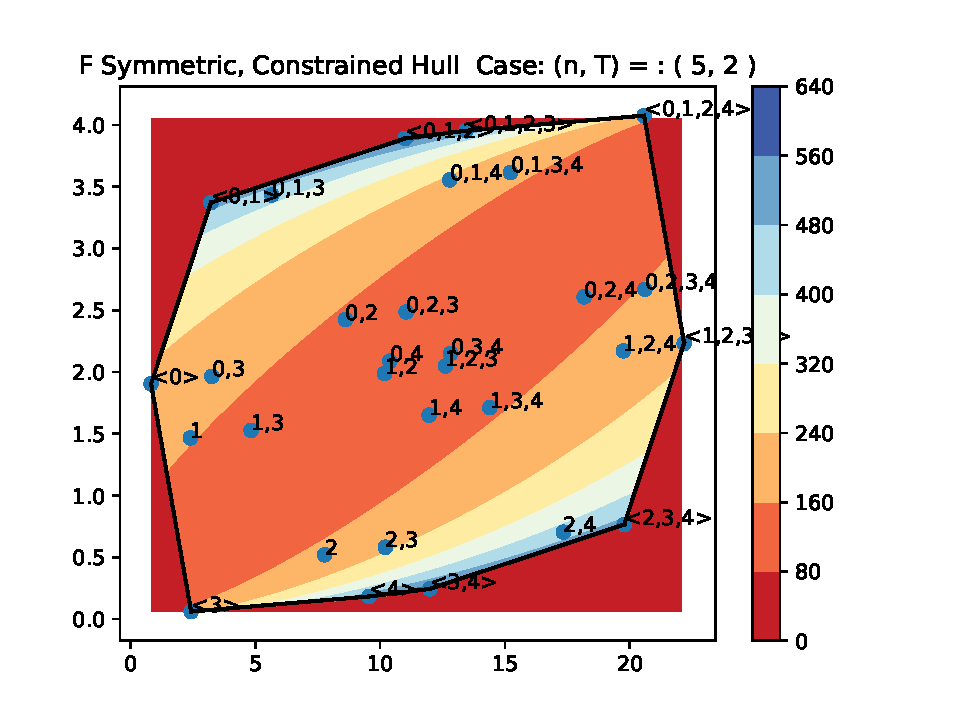
\includegraphics[scale=.55]{const_hull_5_2.pdf}
  \caption{(n,T) = (5,2)}
  \label{fig:sub1}
\end{subfigure}%
\begin{subfigure}{.5\textwidth}
  \centering
  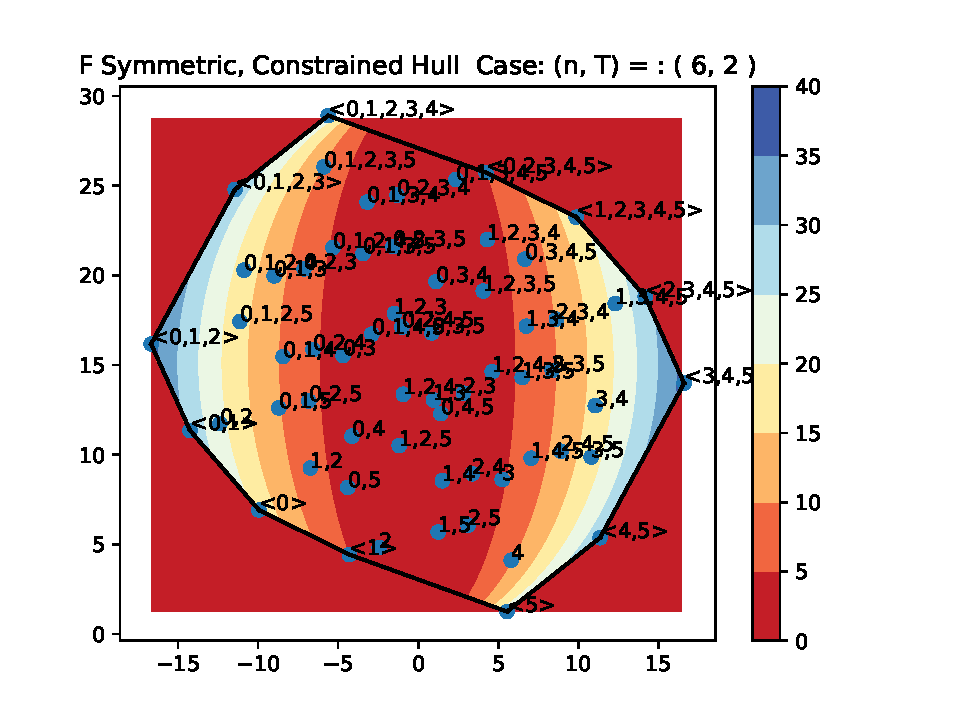
\includegraphics[scale=.55]{const_hull_6_2.pdf}
  \caption{(n,T) = (6,2)}
  \label{fig:sub2}
\end{subfigure}
\caption{Constrained convex hull $\underline{\mathcal{C}}$ for (n,T) = (5,2), (6,2) $N = \left\lbrace 0,1, \dots, n-1 \right\rbrace$ with level sets for the symmetric $\overline{F}$ with $\gamma = 2$. Vertices are labeled by $<>$, and the consecutive splitting partition pair associated with $\left\lbrace 3\right\rbrace$, $\left\lbrace 0, 1, 2, 4\right\rbrace$ lie on the hull in (a), while the the consecutive splitting pair $\left\lbrace 4\right\rbrace$, $\left\lbrace 0, 1, 2, 3, 5\right\rbrace$ lie on the hull in (b).}
\label{fig:hull1}
\end{figure}

\vspace{6pt}
\begin{figure}
\centering
\begin{subfigure}{.5\textwidth}
  \centering
  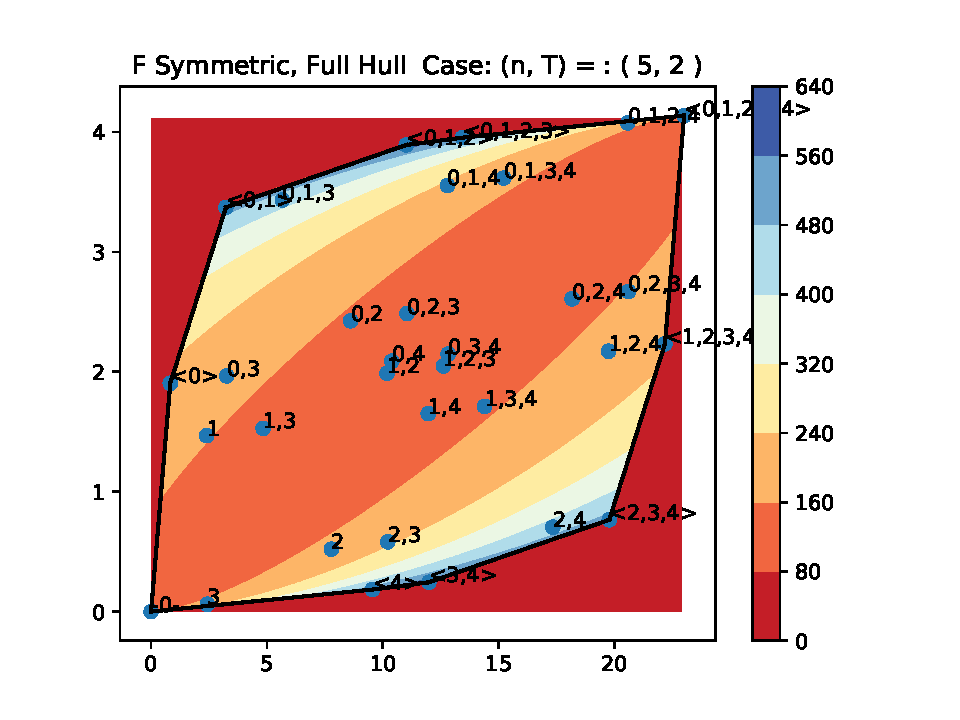
\includegraphics[scale=.55]{full_hull_5_2.pdf}
  \caption{(n,T) = (5,2)}
  \label{fig:sub1}
\end{subfigure}%
\begin{subfigure}{.5\textwidth}
  \centering
  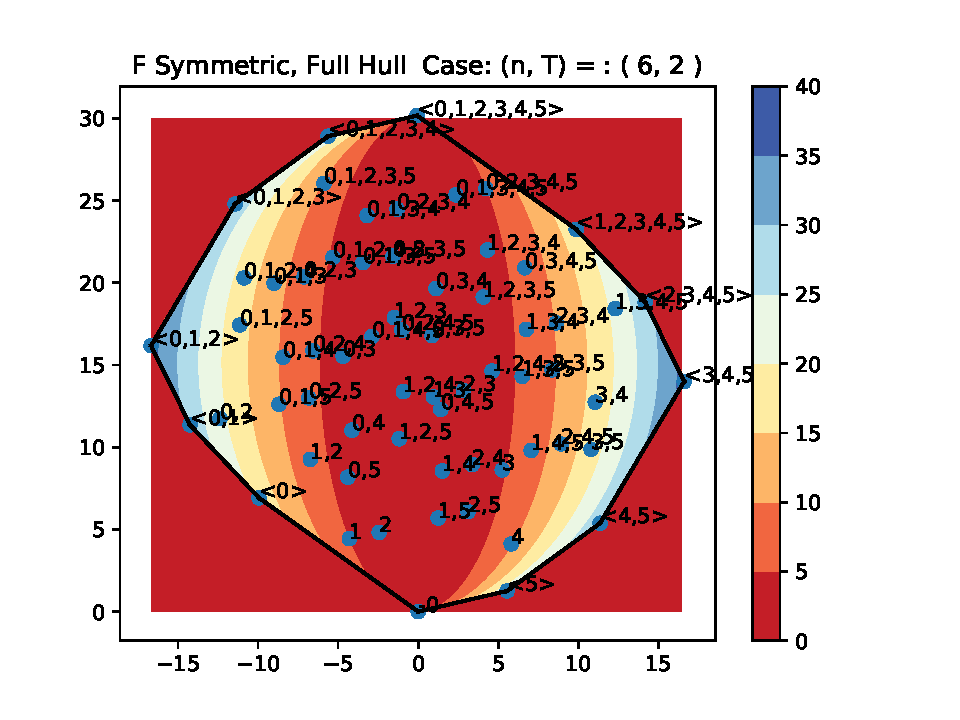
\includegraphics[scale=.55]{full_hull_6_2.pdf}
  \caption{(n,T) = (6,2)}
  \label{fig:sub2}
\end{subfigure}
\caption{Full convex hull for the above cases, only consecutive non-splitting partition points lie on both hulls.}
\label{fig:test}
\end{figure}

From Proposition 1, a convex $F$ will take its maximum on $\underline{mathcal{C}}$ at either a splitting or nonsplitting consecutive partition point. The former case represents a kind of degenerate behavior, associated with the collapsing of weakly consecutive maximal partitions seen in earlier examples. A necessary condition on a relaxed problem can be used to identify this behavior.

\begin{prop}
Let $F$ be a convex score function. If $\argmax_{\left( x,y\right) \in \underline{\mathcal{C}}} \overline{F}\left( x,y\right)$ is splitting, then $p_\mathcal{V} = \argmax_{\left( x,y\right) \in \mathcal{C}} \overline{F}$. If in addition $F$ is positive or bounded below on $\mathcal{C}$ then all of the $x_i$ are of the same sign.
\end{prop}
\begin{proof}
Let $\overline{p} = \argmax_{\left( x,y\right) \in \overline{\mathcal{C}}} \overline{F}\left( x,y\right)$, with $\overline{p}$ consecutive splitting in $\mathcal{V}$. Let $p = \argmax_{\left( x,y,\right) \in \mathcal{C}} \overline{F}\left( x,y\right)$. Convexity of $\overline{F}$ on $\mathcal{C}$ follows from the corresponding property of $F$, so $p \in \mathcal{E}$. Since $\overline{F}\left( p\right) \geq \overline{F}\left( \overline{p}\textsl{•}\right)$, and $\overline{p}$ is not an extreme point of $\mathcal{C}$ by Proposition 1, we have $\overline{F}\left( p\right) > \overline{F}\left( \underline{p}\right)$. So $p$ cannot lie in $\underline{cal{E}}$. The only elements in $\mathcal{E}\setminus \underline{\mathcal{E}}$ are $\left\lbrace p_{\emptyset}, p_{N}\right\rbrace$, so the first part follows. Finally, if $\overline{F}$ is maximaixed at $p_\mathcal{V}$ and there is a $1 \leq q < n$ with $\frac{x_1}{y_1} \leq \dots \leq \frac{x_q}{y_q} \leq 0 \leq \frac{x_{q+1}}{y_{q+1}} \leq \dots \leq \frac{x_n}{y_n}$, then by strict monotonicity of $F$ in $x$, $y$, we have $F\left( \sum_{q+1}^n x_i, \sum_{q+1}^n y_i\right) > F\left( p_\mathcal{V}\right)$, hence $\overline{F}\left( \sum_{q+1}^n x_i, \sum_{q+1}^n y_i\right) > F\left( p_\mathcal{V}\right) = \overline{F}\left( p_\mathcal{V}\right)$, unless $q = 0$ or $q = n$, in which case all of the $x_i$ of the same sign.
\end{proof}


\begin{thm} \label{thm1}
Let the dataset $\mathcal{D} = \{ \mathbf{R}_1, \ldots, \mathbf{R}_n \}$ be ordered with the standard priority function. If the score function $F$ is convex and subadditive, then there is a strongly consecutive maximal partition for $F$, for any $X \subseteq \mathbf{R}$, $Y \subseteq \mathbf{R}$.
\end{thm}

\begin{proof}
The proof proceeds by induction on $t$. Let $t$ = 2. By convexity of $\overline{F}$, the argmax of $\overline{F} |_{\underline{\mathcal{C}}}$ occurs at a point $p_S$, for $S \in \Pi\left( \underline{\mathcal{U}}\right) \cup \Pi\left( \underline{\mathcal{S}}\right)$. Since $F$ is subadditive, the solution to $\argmax_{\mathcal{C}}{\overline{F}}$ cannot occur at $p_{\mathcal{V}}$, hence $p_S \in \Pi\left( \mathcal{U}\right)$ by Proposition 2. So the maximal partition $\left\lbrace S, \mathcal{V} \setminus S\right\rbrace$ is strongly consecutive. Now let $t >= 3$. The arguments here a are motivated by $\cite{article2}$. Define, for any subset $S \subseteq \mathcal{V}$, $M_S = \max S$, $m_S = \min S$, and $d\left(S\right) = M_S - m_S$. Let $\mathcal{P} = \left\lbrace S_1, \dots, S_t\right\rbrace$ be a size $t$ partition that maximizes $\ref{eq1}$ which also minimizes $\sum_{j=1}^t d\left(S_j\right)$ among all optimal size $t$ partitions. If not all $S_j$ are consecutive, then we can find $S_i$, $S_j$ and $k \in S_j$ with $m_{S_i} < k < M_{S_i}$. Note that $\min\left( M_{S_i}, M_{S_j}\right) \geq k$,  and $\max\left( m_{S_i}, m_{S_j} \right) \leq k$, so that 
\[
\min\left( M_{S_i}, M_{S_j}\right) - \max\left( m_{S_i}, m_{S_j} \right) \geq 0.
\] 
By the induction hypothesis, we can find an optimal partition of $S_i \cup S_j$ into nonempty consecutive sets $S^{\prime}_i, S^{\prime}_j$ with respect to $S_i \cup S_j$. Then $d\left( S^{\prime}_i\right) + d\left( S^{\prime}_j\right) \leq \max\left( M_{S_i}, M_{S_j}\right) - \min\left( m_{S_i}, m_{S_j}\right) - 1$, so
\begin{align*}
d\left(S_i\right) + d\left( S_j\right) &= M_{S_i} - m_{S_i} + M_{S_j} - m_{S_j} \\
&= \max\left(M_{S_i}, M_{S_j}\right) + \min\left(M_{S_i}, M_{S_j}\right) \\
&- \min\left( m_{S_i}, m_{S_j} \right) - \max\left( m_{S_i}, m_{S_j} \right) \\
&\geq d\left(S^{\prime}_i\right) + d\left(S^{\prime}_j\right) + 1,
\end{align*}
a contradiction. So all of the $S_j$ are consecutive, nonempty.
\end{proof}

\begin{thm} \label{thm2}
Let the dataset $\mathcal{D} = \{ \mathbf{R}_1, \ldots, \mathbf{R}_n \}$ be ordered with the standard priority function. If the score function $F$ is convex, then there is a weakly consecutive maximal partition for $F$, for any $X \subseteq \mathbf{R}$, $Y \subseteq \mathbf{R}$.
\end{thm}
\begin{proof}
The proof is analagous to the proof of the previous theorem. At the initial step, we can only guarantee that the argmax $p_S$ of $\overline{F} |_{\underline{\mathcal{C}}}$ satisfies $S \in \Pi\left( \underline{\mathcal{U}}\right) \cup \Pi\left( \underline{\mathcal{S}}\right)$, that is, we cannot exclude it from $\Pi\left( \underline{\mathcal{S}}\right)$. The partition formed is nonetheless weakly consecutive. For the remainder, assume $S_i$, $S_j$ are chosen as above, and one of  $S^{\prime}_i$, $S^{\prime}_j$ to be empty, defining $d(\emptyset) = 0$. The argument still holds.
\end{proof}

\begin{corollary}
For $\mathcal{D}$ as above, $F(x,y) = x^{\alpha}y^{-\beta}$ a rational score function. Then for $X \subseteq \mathbf{R}$, a strongly consecutive maximal partition for $F$ exists if $\alpha - \beta = 1$ and $\alpha$ is even, while a weakly consecutive maximal partition exists if $\alpha - \beta = 1$. For $X \subseteq \mathbf{R}^+$, both strongly and weakly consecutive maximal partitions exist if $\alpha - \beta = 1$.
\end{corollary}
\begin{proof}

Show that $F$ is convex iff $\alpha - \beta \geq 1$, with the additional requirement that $\alpha$ is even for general $X$, and $F$ is subadditive iff $\alpha - \beta \leq 1$...
\end{proof}

It is difficult to establish equivalence for the results in $\ref{thm1}$, $\ref{thm2}$, as the extension of the function $F \colon 2^\mathcal{V} \rightarrow \mathbf{R}$ to one on $\underline{\mathcal{C}}$ or $\mathcal{C}$ is not well-defined. The notion of submodularity does not seem to be related - the score function $F(x,y) = \log((1+x)(1+y))$ is submodular, for $X \subseteq \mathbf{R}^+$, but the real valued function defined on the polytope is subadditive and concave. Thus a maximum may occur on the interior of $\underline{\mathcal{C}}$. The Lovasz extension of $F$ is defined on the unit hypercube in $\mathbf{R}^n$, but the natural projections to $\mathbf{R}^2$ that extend $F$ don't preserve convexity. If we restrict attention to rational score functions, then there is an equivalence. For example,  choose $\alpha = 2 + \epsilon$, $\beta = 1$, for some $\epsilon > 0$. Set
\[
X = \left[ 1-\delta, \delta, 1 + \delta\right], Y = \left[ 1, \delta, 1\right]
\] 
for some $\delta > 0$. There are 3 partitions of $\left\lbrace 1, 2, 3\right\rbrace$, namely $\mathcal{P}_1 = \left\lbrace \left[ 0 \right], \left[ 1, 2\right]\right\rbrace$, $\mathcal{P}_2 = \left\lbrace \left[ 0, 1 \right], \left[ 2\right]\right\rbrace$, and $\mathcal{P}_3 = \left\lbrace \left[ 0, 2 \right], \left[ 1 \right]\right\rbrace$. Only the first 2 are ordered. The scores can be computed
\begin{align*}
\text{Score}\left(\mathcal{P}_1\right) & = \left( 1-\delta \right)^\alpha + \frac{\left( 1+2\delta\right)^\alpha}{1+\delta} \\
\text{Score}\left(\mathcal{P}_2\right) & = \frac{1}{1+\delta} + \left( 1+\delta\right)^\alpha \\
\text{Score}\left(\mathcal{P}_3\right) & = 2^{1+\epsilon}
\end{align*}
We can choose $\delta$ small so that the last score dominates.
For $\alpha = 2 - \epsilon$, $\beta = 1$, $\epsilon > 0$, and the sequences
\[
X = \left[ 1, \frac{1}{\delta}, 1\right], Y = \left[ \frac{1}{1+\delta}, \frac{1}{\delta}, \frac{1}{1-\delta}\right]
\] 
we have
\begin{align*}
\text{Score}\left(\mathcal{P}_1\right) & = \frac{1^\alpha}{\frac{1}{1+\delta}} + \frac{\left(1 + \frac{1}{\delta}\right)^\alpha}{\left( \frac{1}{\delta} + \frac{1}{1 - \delta}\right) }  = \frac{\left(1 + \frac{1}{\delta}\right)^\alpha}{\left( \frac{1}{\delta} + \frac{1}{1 - \delta}\right) } + \left( 1 + \delta \right)\\
\text{Score}\left(\mathcal{P}_2\right) & = \frac{1^\alpha}{\frac{1}{1-\delta}} + \frac{\left( 1 + \frac{1}{\delta}\right)^\alpha}{\left( \frac{1}{1+\delta} + \frac{1}{\delta}\right)}  = \frac{\left( 1 + \frac{1}{\delta}\right)^\alpha}{\left( \frac{1}{1+\delta} + \frac{1}{\delta}\right)} + \left( 1 - \delta \right)\\
\text{Score}\left(\mathcal{P}_3\right) & = \frac{\left( 1 + 1\right)^\alpha}{\left(\frac{1}{1+\delta} + \frac{1}{1-\delta}\right)}  + \frac{\left( \frac{1}{\delta}\right)^\alpha}{\frac{1}{\delta}} = \frac{\left( \frac{1}{\delta}\right)^\alpha}{\frac{1}{\delta}} + 2^{\alpha - 1}\left( 1 - \delta^2\right) 
\end{align*}
and letting $\delta \rightarrow 0$ gives the result, as the first summands in each score can be made arbitrarily close to each other.

To extend these examples to larger $\vert \mathcal{D} \vert = n > 3$, $s \geq t$, simply add $n-3$ identical records of the form $R_i = \left( 0, y\right)$, for any $y > 0$. Index the new elements by $N+1, \dots, M$. Since $s \geq t$, an unordered candidate partition is formed by adjoining to $\mathcal{P}^{\prime} = \left[\left[0, 2\right], \left[ 1\right]\right]$ an arbitrary partition $\mathcal{P}^{\prime\prime}$ of size $s - t$ of the indices $4, \dots, n$, the new partition is $\mathcal{P} = \mathcal{P}^{\prime} \cup \mathcal{P}^{\prime\prime}$. We have $\text{Score}\left(\mathcal{P}\right) = \text{Score}\left(\mathcal{P}^{\prime}\right)$. It is clear that inserting any record in any subset of $\mathcal{P}^{\prime\prime}$ into any subset from a partition in $\mathcal{P}^{\prime}$ only decreases the total score, while inserting a record from $\mathcal{P}^{\prime}$ into $\mathcal{P}^{\prime\prime}$ also represents a decrease from one of the above partitions scores for $\mathcal{P}_1$, $\mathcal{P}_2$, if the element of index 1 is switched, nonetheless the new partition won't be ordered. Of the elements 0, 2, the only one that can be switched while retaining an ordered partition is 2, in which case the new partition is of the form $\left[ \left[ 0\right], \left[ 1\right], \left[ 2, \dots\right]\right]$. But the score of any such partition must be less than
\[
\left( 1-\delta\right)^\alpha + \frac{\delta^\alpha}{\delta} + \left( 1+\delta\right)^\alpha
\]
which is dominated by the unordered partition $\mathcal{P}_3 = \left\lbrace \left[ 0, 2 \right], \left[ 1 \right]\right\rbrace$ above. The argument for $\alpha < 2$ is similar. In this way we can generate optimal, unordered partitions for any $\alpha > 0$ and $\left( n, t\right)$. Therefore $\alpha = 2$. This argument can be easily generalized to the cases $\alpha - \beta > 1$ and $\alpha - \beta < 1$. 

In addition for $\alpha = 2$, $\beta = 1$ and priority function $G\left( x,y\right) = \frac{x^{\tau}}{y}$, $\tau = 1$ is the only priority power that guarantees the existence of a strongly consecutive maximal partition. To see this let
\[
X = \left[ x-\delta, \delta, x + \delta\right], Y = \left[ x, \delta, x\right]
\] 
for $x, \delta > 0$, and consider the three partitions $\mathcal{P}_i$, $i=1, 2, 3$ as above. We have
\begin{align*}
& \text{Score}\left(\mathcal{P}_1\right) = \text{Score}\left(\mathcal{P}_2\right) \\
& \text{Score}\left(\mathcal{P}_3\right) - \text{Score}\left(\mathcal{P}_1\right) = \text{Score}\left(\mathcal{P}_3\right) - \text{Score}\left(\mathcal{P}_2\right) = \frac{-\delta^2\left( 2x + \delta\right)}{x\left( x + \delta\right)}
\end{align*}
The power priority $G(x,y) = \frac{x^\tau}{y}$ places the priorty on the records:
\begin{align} \label{eq8}
\left( G(x_1, y_1), G(x_2, y_2), G(x_3, y_3)\right) = \left( \frac{\left( x - \delta \right)^{\tau}}{x}, \delta^{\tau-1},  \frac{\left( x + \delta \right)^{\tau}}{x}\right).
\end{align}
For $\tau > 1$, choosing $x$ large relative to delta gives $G(x_2, y_2) < G(x_1, y_1) < G(x_3, y_3)$. So the partitions $\mathcal{P}_1 = \left\lbrace \left[ 0 \right], \left[ 1, 2\right]\right\rbrace$, $\mathcal{P}_2 = \left\lbrace \left[ 0, 1 \right], \left[ 2\right]\right\rbrace$, and $\mathcal{P}_3 = \left\lbrace \left[ 0, 2 \right], \left[ 1 \right]\right\rbrace$ become $\mathcal{P}_1 = \left\lbrace \left[ 1 \right], \left[ 0, 2\right]\right\rbrace$, $\mathcal{P}_2 = \left\lbrace \left[ 0, 1 \right], \left[ 2\right]\right\rbrace$, and $\mathcal{P}_3 = \left\lbrace \left[ 1, 2 \right], \left[ 0 \right]\right\rbrace$, maintaining the partition scores above. The maximum score is shared by $\mathcal{P}_1$, $\mathcal{P}_2$, the first being unordered. In order to force $\text{Score}\left(\mathcal{P}_1\right) > \text{Score}\left(\mathcal{P}_2\right)$, we perturb the original $X$, $Y$ by
\[
X\left(\epsilon\right) = \left[ x-\delta+\epsilon, \delta, x + \delta\right], Y = \left[ x, \delta, x\right]
\]
and denoting by $\text{Score}\left(\epsilon \right)\left(\mathcal{P}_i \right)$ the score of the partition $\mathcal{P}_i$ on the records $\left\lbrace \left(x\left(\epsilon\right)_1, y_1\right),\left(x\left(\epsilon\right)_2, y_2\right),\left(x\left(\epsilon\right)_3, y_3\right) \right\rbrace$, it follows that
\begin{align*}
\text{Score}\left(\epsilon \right)\left(\mathcal{P}_1 \right) - \text{Score}\left(\mathcal{P}_1 \right) &= \frac{\left( x + \epsilon - \delta\right)^2}{x} - \frac{\left( x - \delta\right)^2}{x} = \frac{2\epsilon\left( x - \delta\right) + \epsilon^2}{x} \\
\text{Score}\left(\epsilon \right)\left(\mathcal{P}_2 \right) - \text{Score}\left(\mathcal{P}_2 \right) &= \frac{\left( x + \epsilon\right)^2}{x + \delta}  - \frac{x^2}{x+\delta}= \frac{2\epsilon x + \epsilon^2}{x+\delta}
\end{align*}
Choosing, e.g. $x = 1$, $\delta = .25$ gives 
\begin{align*}
\text{Score}\left(\epsilon \right)\left(\mathcal{P}_1 \right) - \text{Score}\left(\mathcal{P}_1 \right) &= \frac{3}{2}\epsilon + \epsilon^2 \\
\text{Score}\left(\epsilon \right)\left(\mathcal{P}_2 \right) - \text{Score}\left(\mathcal{P}_2 \right) &= 2\epsilon + \epsilon^2
\end{align*}
By choosing $\epsilon > 0$ small enough, we can ensure that the first term, corresponding to the score of the partition $\left[ \left[ 1\right], \left[ 0, 2\right]\right]$ dominates, while the priority order $G(x_2, y_2) < G(x_1, y_1) < G(x_3, y_3)$ is maintained. The maximal partition in this case is therefore unordered.
For $ 0 \leq \tau < 1$ and the priority function $G(X,Y) = \frac{x^{\tau}}{y}$, choose $x$ large relative to $\delta$ forces the priority ordering $G(x_0, y_0) \leq G(x_2, y_2) \leq G(x_1, y_1)$. So the  highest and second highest records exchange priority ordering, and the partition $\mathcal{P}_1$ stays the same, while $\mathcal{P}_1$ now corresponds to $\left\lbrace \left[ 0, 2\right], \left[ 1\right]\right\rbrace$, $\mathcal{P}_2$ to $\left\lbrace \left[ 0, 1\right], \left[ 2\right]\right\rbrace$, only the last being ordered. Perturbing the original sequences by
\[
X\left(\epsilon\right) = \left[ x-\delta, \delta, x + \delta + \epsilon\right], Y = \left[ x, \delta, x\right]
\]
yields
\begin{align*}
\text{Score}\left(\epsilon \right)\left(\mathcal{P}_1 \right) - \text{Score}\left(\mathcal{P}_2 \right) &= \frac{\left( x + 2\delta + \epsilon\right)^2}{x + \delta}  - \frac{\left( x + 2\delta\right)^2}{x + \delta} = \frac{2\epsilon\left( x + 2\delta\right) + \epsilon^2}{x + \delta} \\
\text{Score}\left(\epsilon \right)\left(\mathcal{P}_2 \right) - \text{Score}\left(\mathcal{P}_1 \right) &= \frac{\left( x + \delta + \epsilon\right)^2}{x} - \frac{\left( x + \delta\right)}{x} = \frac{2\epsilon\left( x + \delta \right) + \epsilon^2}{x} \\
\end{align*}
We choose $\epsilon > 0$ small enough so that the first term dominates, corresponding to the unordered partition. Therefore $\tau = 1$.

\section{Applications}

The approach above provide an alternative proof of the "fast subset scan" (LTSS) property of spatial scan statistics (see $\cite{article6}$). We seek to detect emerging outbreaks - disease, terrorist activity, etc. - based on cross-sectional or time series data of spattial events. In this setting, a data stream of records $\left\lbrace \mathcal{D_t}, \mathcal{D}_{t+1}, \dots \right\rbrace$ is monitored over time at a set of spatial locations $\left\lbrace s_1, s_2, \dots, s_N \right\rbrace$. For each stream $\mathcal{D}_t$ and location $s_j$ the record entries $R^t_j = (x^t_j, y^t_j)$ may represent occurrences of an event and baselines or expectations, respectively. The $y_i$ values could also represent size or population statistics in absence of baselines, while concurrent estimates of baselines could be made using a Bayesian approach, etc. The goal is to compute any spatial regions (unions of the $s_i$) for which occurences are significantly high. Classical clustering techniques seek to find a cluster representation for all data points are not as commmonly used as parametric $\textit{spatial scan statistics}$ methods, which have higher detection power. The methods rely on a parametric specification for the generation of the counts or occurrences $x^t_j$, for fixed $j$, and specify as score function the likelihood ratio statistic which is generally $\theta = \log\left[ \frac{P\left( \mathcal{D} | H_1\right)}{P\left( \mathcal{D}\right | H_0)}\right]$, where $H_0$ represents sampling under the population density, while $H_1$, the alternative represeents sampling with a higher mean. The most common distributional choices are Poisson and Gaussian. The two qualitative specifications of $Y$, as an expectation of occurences, or as a population representation, give rise to two test statistics for each distributional choice. 

The large combinatorial optimization problems resulting from this specification are amenable to a linear-time exact search, referred to as the linear time subset scan property. Specifically, it is shown that the program
\[
\mathcal{S^*} = \argmax_{S \subseteq N} F(\sum_{i \in S}x_i, \sum_{i \in S}y_i)
\]
admits a consecutive subset solution $S^*$ under some mild restrictions on $F$. Our method gives an alternative derivation of the fundamental LTSS result.


\begin{thm} \label{thm3}
[See Theorem 1, $\cite{article6}$] Let $\mathcal{D}$ be a data set of records, and $F$ a quasiconvex score function. Then the solution to
\[
\mathcal{S^*} = \argmax_{S \subseteq N} F(\sum_{i \in S}x_i, \sum_{i \in S}y_i)
\]
is a consecutive nonsplitting subset of $\mathcal{V}$.
\end{thm}
\begin{proof}
Since $F$ is quasiconvex, the solution subset $\argmax F\restriction{\mathcal{C}}$ occurs on an extreme point of $\mathcal{C}$, which by Proposition 1 is consecutive nonsplitting.
\end{proof}

\section{Implementation}
We address a gap in the current literature concerning the case for which $F$ is not subadditive, but admits a weakly maximal consecutive partition. As shown previously, the arguments in $\cite{article1}, \cite{article2}$ only guarantee the existence of maximal weakly consecutive partitions when the score function $F$ is convex in all variables, or quasiconvex. The weakly consecutive partition may have strict size $S$ for $S < T$, and the collapse of size may be complete, to $S = 1$ as we have seen. Any search would require a complete scan of all partitions at level $T$ to find the optimal score, and if the optimal partition is not consecutive, the search would resume at levels $T-1, ...$. There is no efficiency gain unless we know $\textit{a priori}$ that a strict size $S$ optimal consecutive partition exists, or something about the structure of the optimal partition of strict size $T$. We can relax the supermodularity requirment on $F$, obtaining

\begin{thm} \label{thm3}
Let $\mathcal{D}$, $F$, $G$ be as above, with $\tau = 1$. Suppose that $F$ is convex in all arguments. Then for any $1 \leq T \leq N$, there is a maximal strongly singleton splitting partition.
\end{thm}


The brute-force optimization in $\ref{eq1}$ has cost that grows exponentially with $n$. A constrained optimization over the set of all size $T$ ordered partitions has cost that grows as $\binom{n-1}{T-1}$, i.e., as a polynomail of degree $T-1$. In particular, the $T = 2$ problem grows linearly in $n$. There is an improvement that can be made to this approach.

Consider a graph $\mathcal{G} = \left( V, E\right)$ with vertices denoted by $\left( i, j\right)$, for $i \in \left\lbrace 1, \dots, n\right\rbrace$, $j \in \left\lbrace 1, \dots, T\right\rbrace$. Add a source node $\left( 1, 1\right)$ and a terminal sink node labeled $\left( n+1, T+1\right)$, Add directed edges from node $\left( i,k \right)$ to $\left( i, k+1\right)$, for each $i < j$, with edge cost $\frac{-\left(\sum_{r=i}^{j-1} x_r\right)^2}{\sum_{r=i}^{j-1} y_r}$. The interpretation is that a path from node $\left( i, j\right)$ to $\left( k, j+1\right)$ represents choice of the subset $\left\lbrace i, \dots, k\right\rbrace$ as the $i^{th}$ subset in the candidate partition. One can then solve for the shortest path by finding a shortest path by the Bellman-Ford algorithm. 


% 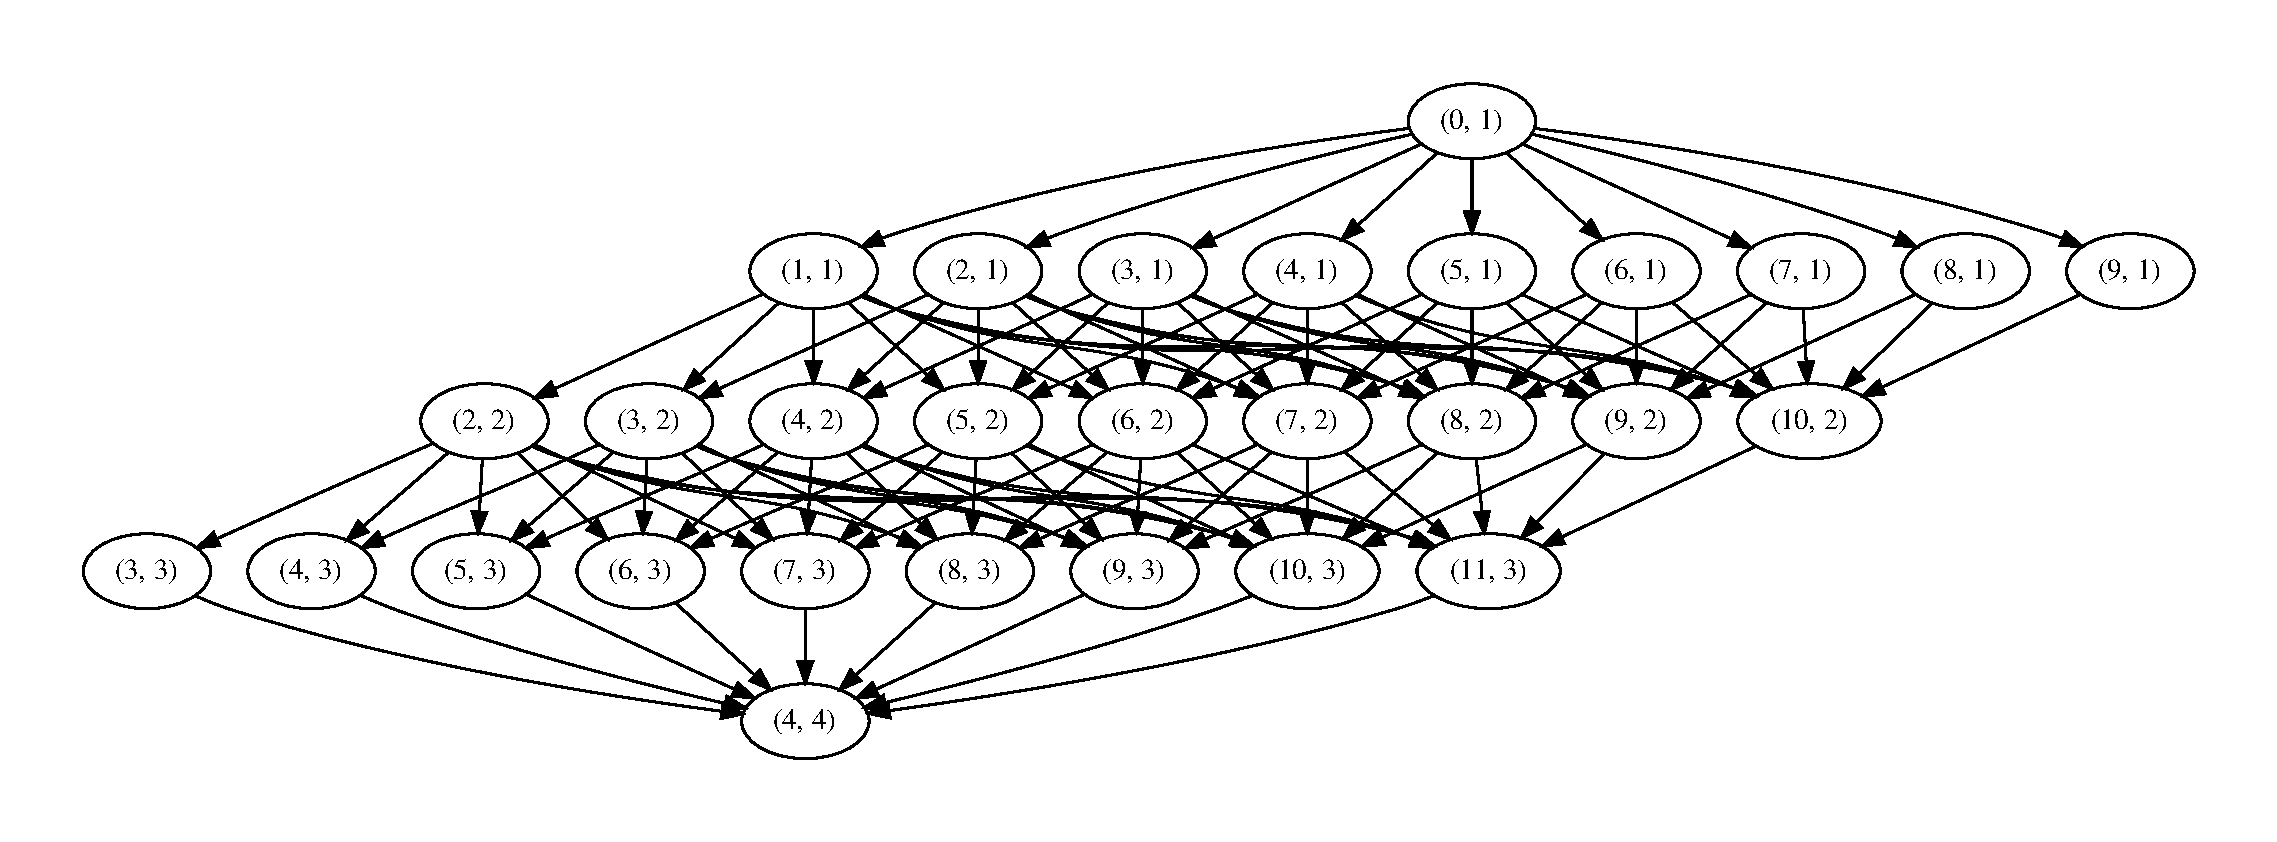
\includepdf[pages=-]{12_4_unlabeled.pdf}
% \begin{figure}
%   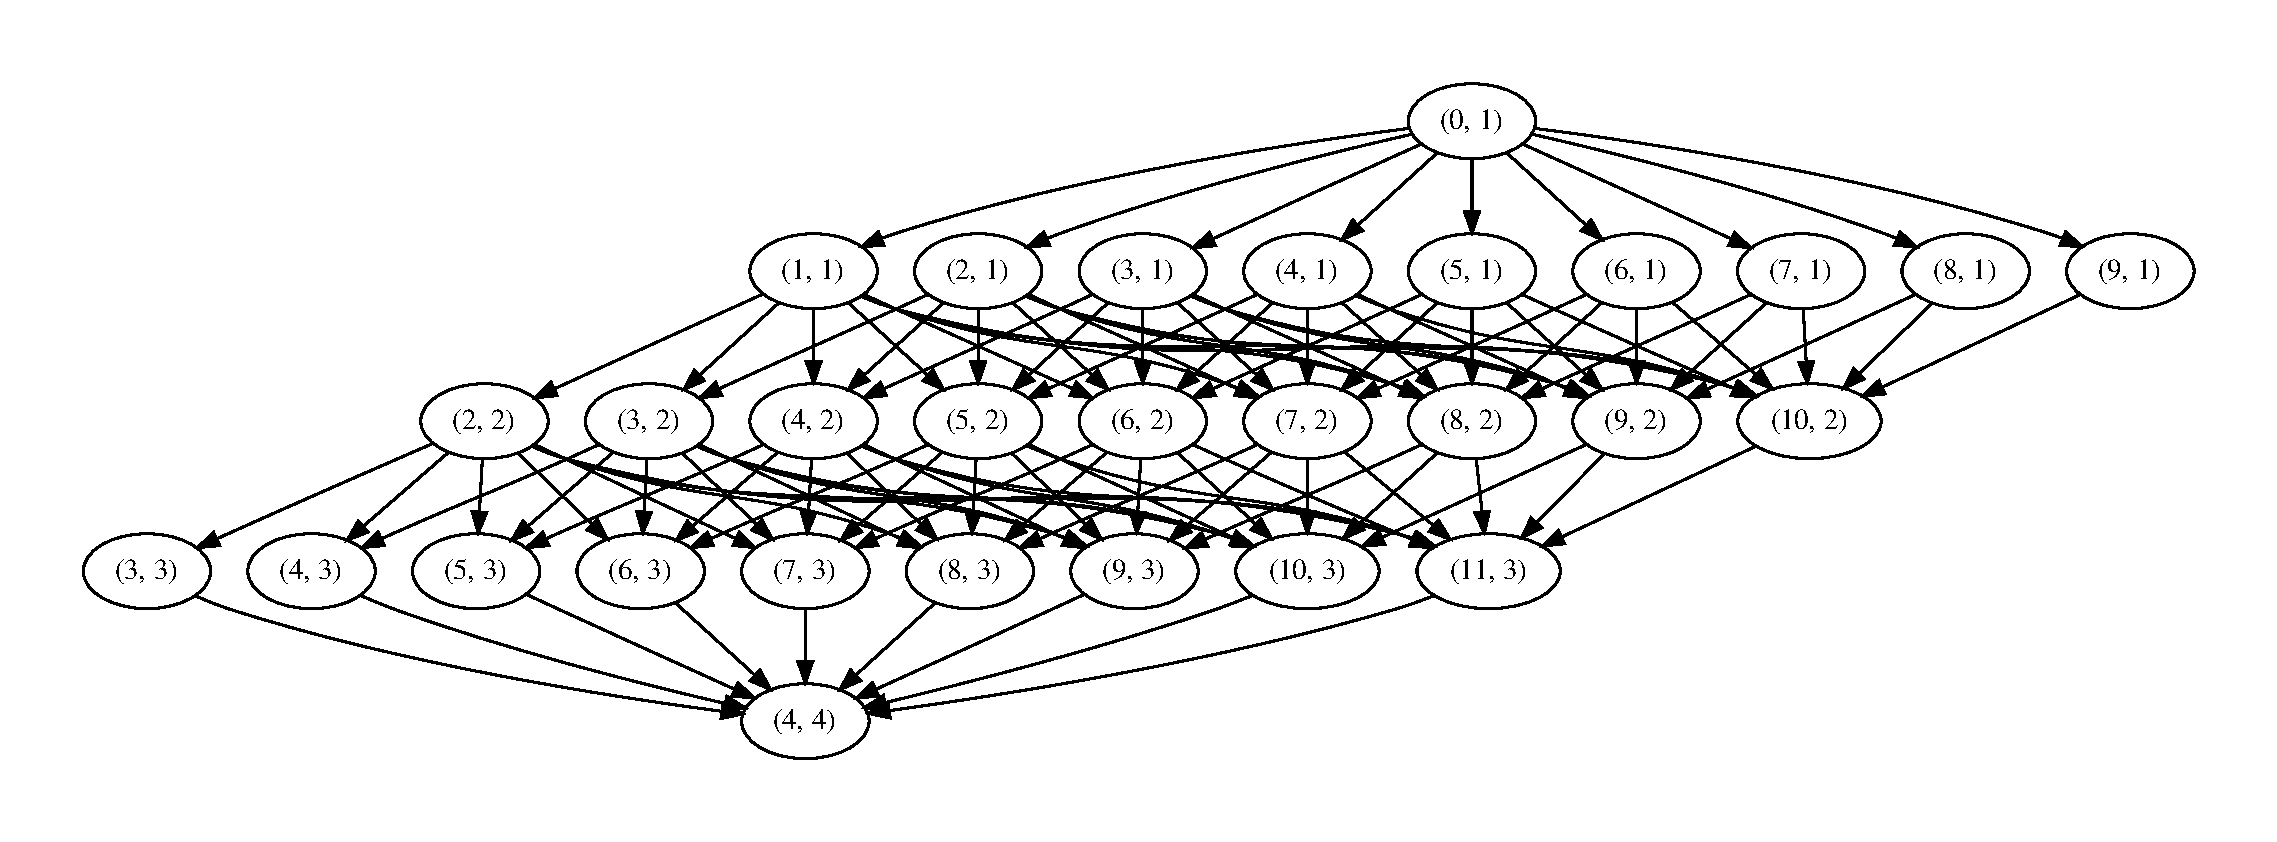
\includegraphics[scale=.22]{12_4_unlabeled.pdf}
%   \caption{Graph connectivity, (N, T) = (12, 4)}  
% \end{figure}

\vspace{16pt}
\begin{figure}
  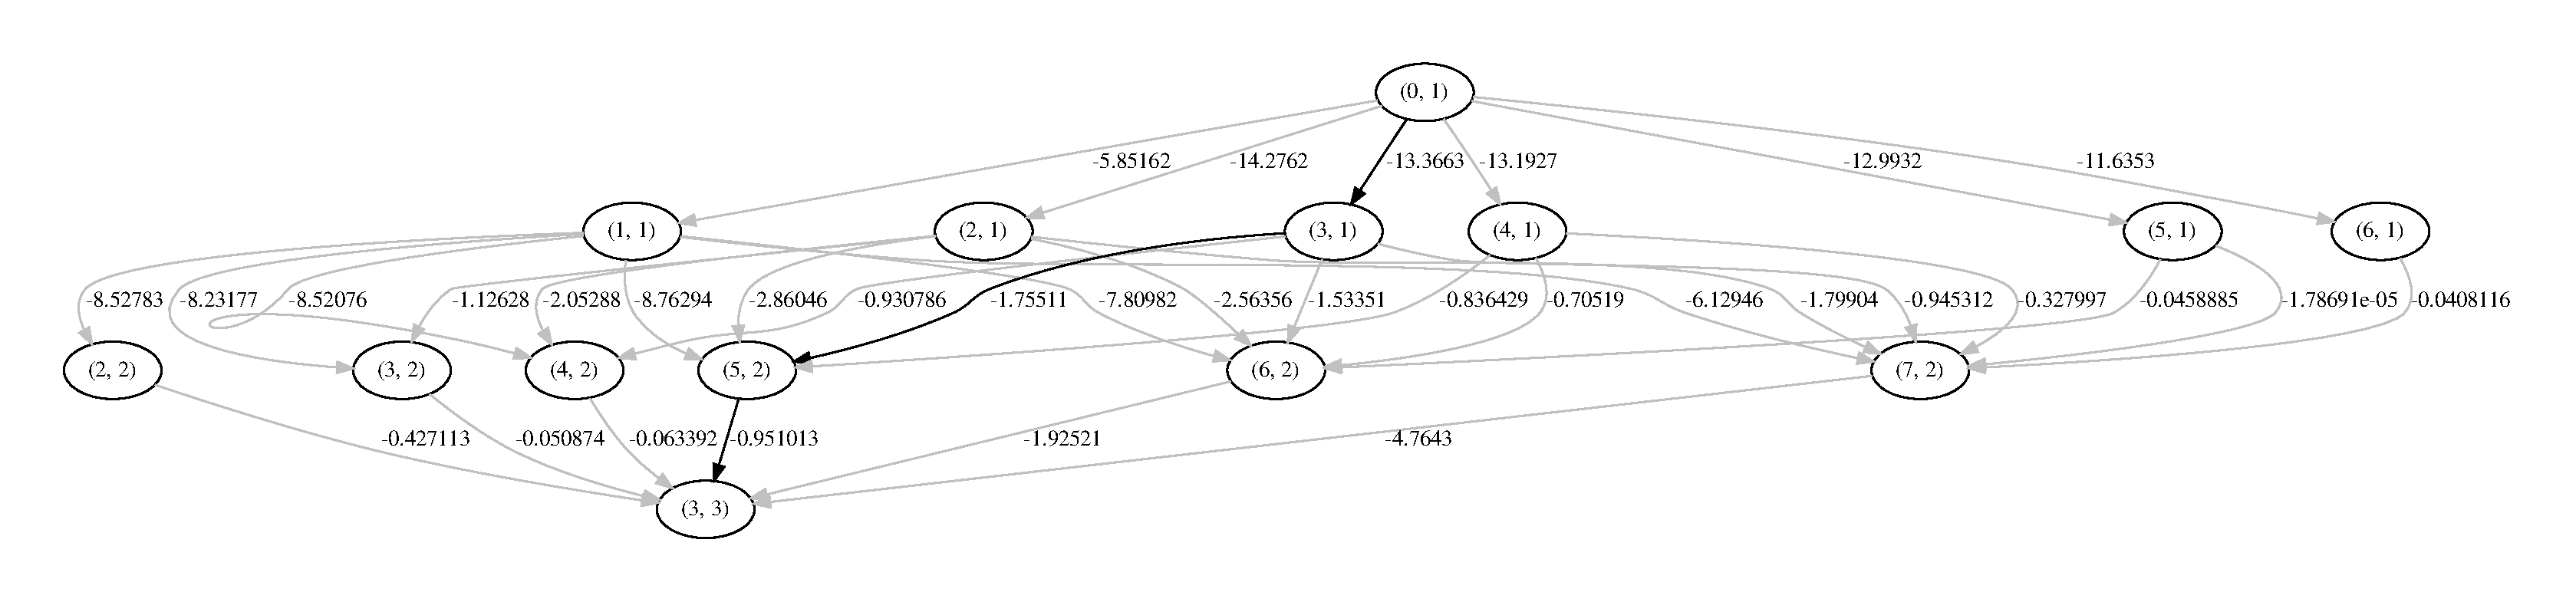
\includegraphics[scale=.25]{8_3_labeled.pdf}
  \caption{Labeled (N, T) = (8, 3) case displaying optimal path SOURCE -- (3, 1) -- (5, 2) --  SINK corresponding to ordered partition [[0 1 2 ], [3 4], [5 6 7 ]]}
\end{figure}

For the graph $\mathcal{G} = \left( V, E\right)$, we have 
\begin{align*}
\vert V \vert & = \left( T-1\right)\left(N-T-1\right) + 2 \\
\vert E \vert & = 2\left( N-T+1\right) + \left( T-1\right)\sum_{i=1}^{N-T+1} i = 2\left( N-T+1\right) + \frac{T-1}{2}\left( N-T+1\right)\left( N-T+2\right)
\end{align*}

The Bellman-Ford algorithm requires $\mathcal{O}\left( V\cdot E\right)$ operations, which for $N >> T$ is $\mathcal{O}\left( TN^2\right)$. A naive search of all ordered partitions requires $\binom{n-1}{T-1}$ operations, a polynomial of order $T-1$ in $N$. We have effectively reduced large cases to be no worse than quadratic in N. The time savings is at the expense of memory footprint; all partial sums of the form $\frac{-\left(\sum_{r=i}^{j-1} x_r\right)^2}{\sum_{r=i}^{j-1} y_r}$ must be stored (although sequential calculation cost is still $\mathcal{O}\left( N\right)$). This may be the most significant feature of this approach - all partial sums are cached on a computation tree that is easily traversed. For example, for a sample size of 10,000 points, with T = 100, there are approximately 4.8530e9 edges, with a storage cost of approximately 19.4119 Gb. Running times are quite fast, however, and we are currently exploring a distributed version of the algorithm.

\cleardoublepage
\appendix
\section{Appendix}
We present here an alternative proof of Theorem 1 which is more in the spirit of $\cite{article6}$, describing and exchange mechanism to swap elements between nonconsecutive subsets that terminates with all subsets consecutive.

\vspace{6pt}

$\textit{Proof of Theorem 1}$
For sufficiency, let $\gamma = 2$, and suppose the partition $\mathcal{P} = \left\lbrace P_1, \dots, P_T\right\rbrace$ is the argmax solution to \ref{eq1}. Let $R_1 = (X_1, Y_1)$ be the set of records in $\mathcal{P}$ that contains the maximal element $R_{(1)}$ of $\mathcal{D}$, and define $R_1^{in} = \argmin_{R_j \in X_1} G(x_i, y_i)$, $R_1^{out} = \argmax_{R_j \not\in X_1} G(x_i, y_i)$. Note that $X_1$ is an ordered subset if and only if $R_1^{in} <= R_1^{out}$, so that there are no "holes" in $X_1$. This is not true if $X_1$ does not contain the maximal element. This can be made precise by defining $I_1^{in} = j \text{ such that} R_{(j)} = R_1^{in}$, $I_1^{out} = j \text{ such that} R_{(j)} = R_1^{out}$, and $D_1 = I_1^{in} - I_1^{out}$. It is then the case that $D_1 \geq 1$, and $X_1$ is ordered if and only iff $D_1 < 0$.

Set $D = D_1$ and assume $D_1 \geq 0$. We describe an iterative procedure that swaps elements between $X_1$ and the remaining subsets, such that each step does not decrease the overall score of the partition, and decreases the value of $D$ by at least 1. In this way the procedure can be stopped when $X_1$ is ordered. We can then remove $X_1$ from the partition, regarding the remaining subsets as a partition of $\left\lbrace 1, \dots N-\vert X_1 \vert\right\rbrace$, and apply the same procedure to the remaining subset containing the maximal element. The process terminates with a maximal ordered partition.

\begin{algorithm}
\caption{Ordering Algorithm: Single Subset}
\begin{algorithmic}[1]
\State $\textit{Select } X_1 \textit{ containing maximal element of } \mathcal{D}$
\State $\left( \alpha , \beta \right) \gets R_1^{in}, \left( a,b \right) \gets R_1^{out}$
\State $D \gets I_1^{in} - I_1^{out}$
\While{$D \geq 0$}
\If{$X_1, X_2 \geq 0$}
\State $X_1^\prime \gets X_1\setminus \left\lbrace x_1^{in}\right\rbrace$, $Y_1^{\prime} \gets X_1\setminus \left\lbrace y_1^{in}\right\rbrace$
\State $X_2^{\prime} \gets X_2\cup \left\lbrace x_1^{in}\right\rbrace$, $Y_2^{\prime} \gets X_2\cup \left\lbrace y_1^{in}\right\rbrace$
\EndIf
\If{$X_1, X_2 \leq 0$}
\State $X_1^{\prime\prime} \gets X_1\cup \left\lbrace x_1^{out}\right\rbrace$, $Y_1^{\prime\prime} \gets X_1\cup \left\lbrace y_1^{out}\right\rbrace$
\State $X_2^{\prime\prime} \gets X_2\setminus \left\lbrace x_1^{out}\right\rbrace$, $Y_2^{\prime\prime} \gets X_2\setminus \left\lbrace y_1^{out}\right\rbrace$
\EndIf
\If{$X_1 \leq 0, X_2 \geq 0 \textit{ or } r X_1 \geq 0, X_2 \leq 0$}
\State $\left\lbrace X_1, Y_1, X_2, Y_2 \right\rbrace \gets \textit{one of } \left\lbrace X_1^{\prime}, Y_1^{\prime}, X_2^{\prime}, Y_2^{\prime}\right\rbrace, \left\lbrace X_1^{\prime\prime}, Y_1^{\prime\prime}, X_2^{\prime\prime}, Y_2^{\prime\prime}\right(\rbrace$
\EndIf
\State {$D \gets I_1^{in} - I_1^{out}$}
\EndWhile
\end{algorithmic}
\end{algorithm}

Without loss of generality, assume $R_1^{out} \in X_2$. We will assume that $G(x_1^{in}, y_1^{in}) < G(x_1^{out}, y_1^{out})$, and show that we can obtain an improvement in the sum $F(X_1, Y_1) + F(X_2, Y_2)$ by exchanging elements of $X_1$, $X_2$. In this way the elements of the subset $X_1$ are sucessively swapped out until it is ordered. Since $X_1$ is the partition with maximal element, we can remove it from consideration, and find the maximal remaining element, and apply the same procedure. In this way we obtain a partition all of whose subsets are ordered.

Assume the tuples $R_1^{in}$, $R_1^{out}$ are composed of $R_1^{in} = \left(x_1^{in}, y_1^{in}\right), R_1^{out} = \left(x_1^{out}, y_1^{out}\right)$.

Define
\begin{align*}
X^\prime\left( \lambda \right) & = \lambda \left( X_1 - x_1^{in}\right) + \left( 1 - \lambda\right) \left( X_1^\prime + x_1^{out}\right) \\
Y^\prime\left( \lambda \right) & = \lambda \left( Y_1 - y_1^{in}\right) + \left( 1 - \lambda\right) \left( Y_1^\prime + y_1^{out}\right)
\end{align*}

for $\lambda \in \left[ 0,1\right]$. For $\lambda_{*} = \frac{y_1^{out}}{y_1^{in} + y_1^{out}}$, we have $Y^\prime\left( \lambda_{*}\right) = Y_1$, and 
\[X^\prime\left( \lambda_{*}\right) = X_1 + \frac{y_1^{in}x_1^{out}-y_1^{out}x_1^{in}}{y_1^{in} + y_1^{out}}\]

Since $G(x_1^{in}, y_1^{in}) < G(x_1^{out}, y_1^{out})$, $\frac{y_1^{in}x_1^{out}-y_1^{out}x_1^{in}}{y_1^{in} + y_1^{out}} > 0$ and $X^\prime\left( \lambda_{*}\right) > 0$. We therefore have 
\begin{align} \label{eq2}
F(X_1, Y_1) \leq F(X^\prime\left( \lambda \right), Y_1) \leq \lambda\left( F(X_1-x_1^{in},Y_1-y_1^{in})\right) + \left( 1 + \lambda\right)\left( F(X_1+x_1^{out},Y_1+y_1^{out})\right)
\end{align}
where the second inequality is from the quasiconvexity of $F$ for $\gamma = 2$. From \ref{eq2} it follows that 
\begin{align} \label{eq3}
F(X_1, Y_1) \leq \max{\left(F(X_1-x_1^{in},Y_1-y_1^{in}), F(X_1+x_1^{out},Y_1+y_1^{out})\right)}
\end{align}

To get a similar result for the sets $X_2$, $Y_2$, define the transformed sequences $\bar{X} = \left\lbrace -x_1, \dots, -x_n\right\rbrace$, $\bar{Y} = \left\lbrace y_1, \dots, y_n\right\rbrace$. The sets $\bar{X_1}, \bar{X_2}, \bar{Y_1}, \bar{Y_2}$ are similarly defined, and we can define $\bar{R_2}^{in} = \argmin_{\bar{R_j} \in \bar{X_2}} G(\bar{x_i}, \bar{y_i})$, $\bar{R_1}^{out} = \argmax_{\bar{R_j} \not\in \bar{X_1}} G(\bar{x_i}, \bar{y_i})$. Assuming the correspondence between record and underlying sequences $\bar{R}_i = \left(\bar{x_i}, \bar{y_i}\right)$, we then have $x_1^{in} = -\bar{x}_2^{out}$, $y_1^{in} = \bar{y_2}^{out}$, and $x_1^{out} = -\bar{x}_2^{in}$, $y_1^{out} = \bar{y_2}^{in}$. 

Define
\begin{align*}
\bar{X}^\prime\left( \lambda \right) & = \lambda \left( \bar{X_2} - \bar{x_2}^{in}\right) + \left( 1 - \lambda\right) \left( \bar{X_2} + \bar{x_2}^{out}\right) \\
\bar{Y}^\prime\left( \lambda \right) & = \lambda \left( \bar{Y_2} - \bar{y_2}^{in}\right) + \left( 1 - \lambda\right) \left( \bar{Y_2} + \bar{y_2}^{out}\right)
\end{align*}

for $\lambda \in \left[ 0,1\right]$. For $\bar{\lambda}_{*} = \frac{\bar{y_2}^{out}}{\bar{y_2}^{in} + \bar{y_2}^{out}}$, we have $\bar{Y}^\prime\left( \bar{\lambda}_{*}\right) = \bar{Y_1}$, and 
\[\bar{X}^\prime\left( \bar{\lambda}_{*}\right) = \bar{X_2} + \frac{\bar{y_2}^{in}\bar{x_2}^{out}-\bar{y_2}^{out}\bar{x_2}^{in}}{\bar{y_2}^{in} + \bar{y_2}^{out}}\]
By similar arguments, and since $\bar{y_2}^{in}\bar{x_2}^{out}-\bar{y_2}^{out}\bar{x_2}^{in} = x_1^{out}y_1^{in} - x_1^{in}y_1^{out} \geq 0$, 
\begin{align*}
F(X_2, Y_2) = F(\bar{X_2}, \bar{Y_2}) & \leq \max{\left(F(\bar{X_2}-\bar{x_2}^{in},\bar{Y_2}-\bar{y_2}^{in}), F(\bar{X_2}+\bar{x_2}^{out},\bar{Y_2}+\bar{y_2}^{out})\right)} \\
& = \max{\left(F(\bar{X_2}-\bar{x_2}^{in},Y_2-y_1^{our}), F(\bar{X_2}+\bar{x_2}^{out},\bar{Y_2}+y_2^{out})\right)} \\
& = \max{\left(F(\bar{X_2} +x_1^{out},Y_2-y_1^{out}), F(\bar{X_2}-x_1^{in},Y_2+y_2^{out})\right)} \\
& = \max{\left(F(X_2 -x_1^{out},Y_2-y_1^{out}), F(X_2+x_1^{in},Y_2+y_2^{out})\right)}
\end{align*}

So
\begin{align} \label{eq4}
F(X_2, Y_2) \leq \max{\left(F(X_2-x_1^{out},Y_2-y_1^{out}), F(X_2+x_1^{in},Y_2+y_1^{in})\right)}
\end{align}

If we form the table
\[
\begin{pmatrix}
&F(X_1 - x_1^{in}, Y_1 - y_1^{in}) & F(X_2 + x_1^{in}, Y_2 + y_1^{in}) \\
&F(X_1 + x_1^{out}, Y_1 + y_1^{out}) & F(X_2 - x_1^{out}, Y_2 - y_1^{out})
\end{pmatrix} = \begin{pmatrix}
&A_{11} & A_{12} \\
&A_{21} & A_{22}
\end{pmatrix}
\]
then the results in \ref{eq2}, \ref{eq4} imply that $F(X_1, Y_1) \leq \max{\left(A_{11}, A_{21}\right)}$ and $F(X_2, Y_2) \leq \max{\left(A_{12}, A_{22}\right)}$. What we would like to show is that $F(X_1, Y_1) + F(X_2, Y_2) \leq \max{\left(A_{11}, A_{12}\right)}$ or $F(X_1, Y_1) + F(X_2, Y_2) \leq \max{\left(A_{21}, A_{22}\right)}$, as those operations represent a swap of records between the two sets $X_1$, $X_2$. To this end assume that the maximum values down columns occur in different rows, e.g. $\max{\left(A_{11}, A_{21}\right)} = A_{11}$, $\max{\left(A_{12}, A_{22}\right)} = A_{22}$. The case for which the maximums occur on the opposite diagonal is handled similarly. We can then assume that 
\begin{align}
& F(X_1 - x_1^{in}, Y_1 - y_1^{in}) - F(X_1, Y_1) \geq 0 \\
& F(X_2 - x_1^{out}, Y_2 - y_1^{out}) - F(X_2, Y_2) \geq 0 \\
& F(X_1 + x_1^{out}, Y_1 + y_1^{out}) - F(X_1, Y_1) \leq 0 \\
& F(X_2 + x_1^{in}, Y_2 + y_1^{in}) - F(X_2, Y_2) \leq 0
\end{align}

Expand 
\[
F(X - \alpha, Y - \beta) - F(X, Y) = \frac{\beta X^2 - 2\alpha XY + \alpha^2 Y}{Y\left( Y-\beta\right)}
\]
and write
\begin{align*}
F(X_1 - x_1^{in}, Y_1 - y_1^{in}) + F(X_2 + x_1^{in}, Y_2 + y_1^{in}) - \left( F(X_1, Y_1) + F(X_2, Y_2)\right) = \\
\left( F(X_1 - x_1^{in}, Y_1 - y_1^{in}) - F(X_1 - x_1^{in}, Y_1)\right) + \left( F(X_1 - x_1^{in}, Y_1) - F(X_1 , Y_1)\right) + \\
\left( F(X_2 + x_1^{in}, Y_2 + y_1^{in}) - F(X_2 + x_1^{in}, Y_2)\right) + \left( F(X_2 + x_1^{in}, Y_2) - F(X_2, Y_2)\right)
\end{align*}

and
\begin{align*}
F(X_1 + x_1^{out}, Y_1 + y_1^{out}) + F(X_2 - x_1^{out}, Y_2 - y_1^{out}) - \left( F(X_1, Y_1) + F(X_2, Y_2)\right) = \\
\left( F(X_1 + x_1^{out}, Y_1 + y_1^{out}) - F(X_1 + x_1^{out}, Y_1)\right) + \left( F(X_1 + x_1^{out}, Y_1) - F(X_1 , Y_1)\right) + \\
\left( F(X_2 - x_1^{out}, Y_2 - y_1^{out}) - F(X_2 - x_1^{out}, Y_2)\right) + \left( F(X_2 - x_1^{out}, Y_2) - F(X_2, Y_2)\right)
\end{align*}

For ease of notation designate $\alpha = x_1^{in}$, $\beta = y_1^{in}$, $a = x_1^{out}$, $b = y_1^{out}$.

The summands for the top equation can then be written
\begin{align*}
s_1 & = \frac{\left(X_1 - \alpha\right)^2\beta}{Y_1\left( Y_1 - \beta\right)} \\
s_2 & = \frac{\alpha \left( \alpha - 2X_1\right)}{Y_1} \\
s_3 & = \frac{-\left( X_2 + \alpha\right)^2\beta}{Y_2\left( Y_2 + \beta\right)} \\
s_4 & = \frac{\alpha\left( \alpha + 2X_2\right)}{Y_2}
\end{align*}

and the bottom
\begin{align*}
t_1 & = \frac{-\left( X_1 + a\right)^2 b}{Y_1\left( Y_1 + b\right)} \\
t_2 & = \frac{a\left( a + 2X_1\right)}{Y_1} \\
t_3 & = \frac{\left( X_2 - a\right)^2b}{Y_2\left( Y_2 - b\right)} \\
t_4 & = \frac{a\left( a - 2X_2\right)}{Y_2}
\end{align*}

We will show that the that one of
\begin{align} \label{eq5}
F(X_1 - \alpha, Y_1 - \beta) + F(X_2 + \alpha, Y_2 + \beta) - F(X_1, Y_1) - F(X_2, Y_2) & \geq 0 \\
F(X_1 + a, Y_2 +b) + F(X_2 - a, Y_2 - b) - F(X_1, Y_1) - F(X_2, Y_2) & \geq 0
\end{align}
holds.


\begin{case} 
$X_1 >= 0$, $X_2 >= 0$. 
\end{case}
We will show that the top row in \ref{eq5} is positive.

\vspace{12pt}

\begin{claim}
$\frac{X_1}{Y_1} \geq \frac{X_2}{Y_2}$, $\frac{X_1}{Y_1} \geq \frac{2a}{b}$, $\frac{X_2}{Y_2} \geq \frac{2\alpha }{\beta}$.
\end{claim}
\begin{claimproof}
Since $F(X - \alpha, Y - \beta) - F(X, Y) = \frac{\beta X^2 - 2\alpha XY + \alpha^2 Y}{Y\left( Y-\beta\right)}$ is a polynomial in $X$, we have
\begin{align*}
F(X_1+a, Y_1+b) - F(X_1,Y_1) \leq 0 & \implies X_1 \not \in \left( \frac{a}{b}Y_1 \pm \vert \frac{a}{b} \vert \sqrt{Y_1\left( Y_1+b\right) } \right) \\
& \implies \frac{X_1}{Y_1} \not \in \left( \frac{a}{b} \left( 1 \pm \frac{\sqrt{Y_1\left( Y_1+b\right) }}{Y_1}\right) \right)
\end{align*}
Since $\frac{X_1}{Y_1} \geq 0$, it follows that $\frac{X_1}{Y_1} \geq \frac{2a}{b}$. By similar reasoning, 
\begin{align*}
F(X_2+\alpha, Y_2+\beta) - F(X_2,Y_2) \leq 0 & \implies X_2 \not \in \left( \frac{\alpha}{\beta}Y_2 \pm \vert \frac{\alpha}{\beta} \vert \sqrt{Y_2\left( Y_2+\beta \right) } \right) \\
& \implies \frac{X_2}{Y_2} \not \in \left( \frac{\alpha}{\beta} \left( 1 \pm \frac{\sqrt{Y_2\left( Y_2+\beta \right) }}{Y_2}\right) \right)
\end{align*}
so that $\frac{X_2}{Y_2} \geq \frac{2\alpha}{\beta}$. Now since $\frac{2\alpha}{\beta} \leq \frac{X_1}{Y_2}$ and $\frac{\alpha}{\beta} \leq \frac{a}{b}$, it follows that $\frac{X_1}{Y_1} \geq \frac{X_2}{Y_2}$.
\end{claimproof}

\begin{claim}
$s_1 + s_3 \geq 0$
\end{claim}
\begin{claimproof}
\begin{align*}
s_1 = \frac{\left( X_1 - \alpha \right)^2\beta }{Y_1\left( Y_1 - \beta\right)} & = \frac{\beta}{Y_1-\beta}F(X_1+\alpha, Y_1) \\
s_3 = -\frac{\left( X_2 + \alpha \right)^2 \beta }{Y_2\left( Y_2+\beta\right) } & = \frac{-\beta}{Y_2 + \beta}F(X_2+\alpha, Y_2)
\end{align*}
So
\begin{align*}
s_1 + s_3 & = \frac{\beta}{Y_1-\beta}F(X_1+\alpha, Y_1) - \frac{\beta}{Y_2 + \beta}F(X_2+\alpha, Y_2) \\
& = \frac{\beta}{Y_1 - \beta}\left( F(X_1, Y_1) + s_2\right) - \frac{\beta}{Y_2 + \beta}\left( F(X_2,Y_2) + s_4\right)
\end{align*}
Since $F(X - \alpha, Y - \beta) - F(X, Y) = \frac{\beta X^2 - 2\alpha XY + \alpha^2 Y}{Y\left( Y-\beta\right)}$, 
\begin{align*}
F(X_1 - \alpha, Y_1 - \beta) - F(X_1, Y_1) \geq 0 & \implies \beta \geq \frac{\alpha Y_1}{X_1^2}\left( 2X_1 - \alpha \right) \implies s_2 \geq -\frac{\beta}{Y_1}F(X_1, Y_1) \\
F(X_2+\alpha, Y_2+\beta) - F(X_2, Y_2) \leq 0 & \implies \beta \geq \frac{Y_2}{X_2^2}\left( 2X_2 + \alpha \right) \implies s_4 \leq \frac{\beta}{Y_2}F(X_2, Y_2)
\end{align*}
So 
\begin{align*}
s_1 + s_3 & \geq \frac{\beta}{Y_1 - \beta}\left( F(X_1, Y_1) - \frac{\beta}{Y_1}F(X_1, Y_1)\right) - \frac{\beta}{Y_2+\beta}\left( F(X_2, Y_2) + \frac{\beta}{Y_2}F(X_2, Y_2)\right) \\
& = \frac{\beta}{Y_1}F(X_1, Y_1) - \frac{\beta}{Y_2}F(X_2, Y_2) \\
& = \beta \left( \left( \frac{X_1}{Y_1}\right)^2 - \left( \frac{X_2}{Y_2}\right)^2 \right) \\
& \geq 0,
\end{align*}
by the previous claim, and that all quantities are positive.

\end{claimproof}
\begin{claim}
$\sum_{i=1}^{4} s_i \geq 0$
\end{claim}
\begin{claimproof}
\begin{align*}
s_2 + s_4 & = F(X_1 +\alpha, Y_1) - F(X_1, Y_1) + F(X_2 + \alpha, Y_2) - F(X_2, Y_2) \\
& = \frac{\alpha \left( \alpha - 2X_1\right)}{Y_1} + \frac{\alpha \left( \alpha + 2X_2\right)}{Y_2}
\end{align*}
As a polynomial in $\alpha$ we have
\[
s_2 + s_4 = p(\alpha) = \alpha \left( g + \frac{1}{2}h \alpha \right),
\]
where
\begin{align*}
g & = \frac{2 \left( X_2 Y_1 - X_1 Y_2\right)}{Y_1 Y_2} \\
h & = \frac{Y_1 + Y_2}{Y_1 Y_2}
\end{align*}
So $p$ has two real roots, one at $\alpha_1 = 0$ and one for $\alpha_2 \geq 0$. The graph is an upward parabola so that $p \geq 0$ for $\alpha \leq 0$, so the remaining case is $\alpha > 0$. We have, as above
\begin{align*}
F(X_1-\alpha, Y_1-\beta) - F(X_1, Y_1) \geq 0 & \implies \alpha \not \in \left( X_1 \pm \vert X_1\vert \sqrt{\frac{Y_1-\beta}{Y_1}}\right) \\
F(X_2+\alpha, Y_2+\beta) - F(X_2, Y_2) \leq 0 & \implies \alpha \not \in \left( -X_2 \pm \vert X_2\vert \sqrt{\frac{Y_2 +\beta}{Y_2}} \right)
\end{align*}
so that $\alpha > 0$ means that $\alpha \in \left[ 0, \min{X_1\left( 1 - \sqrt{\frac{Y_1-\beta}{Y_1}}\right), X_2\left( \sqrt{\frac{Y_2 + \beta}{Y_2} - 1} \right)}\right]$. The idea is that $\alpha$ is small relative to $\beta$ so that the polynomial $p(\alpha) = s_2 + s_4$ never goes negative enough to violate $s_1 + s_2 \leq -\left( s_1 + s_3\right)$. The proof is technical and is below.
\end{claimproof}

\begin{lemma}
For $X_1$, $X_2 > 0$, $alpha \geq 0$, $s1 + s3 \geq 0$, we have $\sum_i s_i \geq 0$
\end{lemma}
\begin{proof}
We can write
\begin{align*}
s_2 + s_4 & = \frac{\alpha \left( \alpha - 2X_1\right)}{Y_1}  + \frac{\alpha\left( \alpha + 2X_2\right)}{Y_2} \\
& = \left( \frac{Y_1}{Y_2} + \frac{Y_2}{Y_1}\right)\alpha^2 + 2\left( \frac{X_2}{Y_2} - \frac{X_1}{Y_1} \right)\alpha
\end{align*}
By the proof of the claim tha $s_1 + s_3 \geq 0$, we have that $s_1 + s_3 \geq \beta \left( \left( \frac{X_1}{Y_1}\right)^2 - \left( \frac{X_2}{Y_2}\right)^2 \right)$, so it is sufficient to show that
\[
\left( \frac{Y_1}{Y_2} + \frac{Y_2}{Y_1}\right)\alpha^2 + 2\left( \frac{X_2}{Y_2} - \frac{X_1}{Y_1} \right)\alpha \geq  - \beta\left( \left( \frac{X_1}{Y_1}\right)^2 - \left( \frac{X_2}{Y_2}\right)^2 \right)
\]
Writing the left-hand side as $q\left( \alpha \right) = h\alpha^2 + g\alpha + c$, it is sufficient to show that $\vert \alpha\vert \vert g + h \alpha\vert \leq \vert \beta\left( \left( \frac{X_1}{Y_1}\right)^2 - \left( \frac{X_2}{Y_2}\right)^2 \right) \vert$. By elementary methods, and the fact that 
\begin{align*}
F(X_1-\alpha, Y_1-\beta) - F(X_1, Y_1) \geq 0 & \implies \alpha \not \in \left( X_1 \pm \vert X_1\vert \sqrt{\frac{Y_1-\beta}{Y_1}}\right) \\
F(X_2+\alpha, Y_2+\beta) - F(X_2, Y_2) \leq 0 & \implies \alpha \not \in \left( -X_2 \pm \vert X_2\vert \sqrt{\frac{Y_2 +\beta}{Y_2}} \right)
\end{align*}
so that $\alpha > 0$ means that $\alpha \in \left[ 0, \min{X_1\left( 1 - \sqrt{\frac{Y_1-\beta}{Y_1}}\right)}\right]$, it can be shown that since $h \leq 0$, $g \geq 0$, $\vert \alpha\vert \vert g + h \alpha\vert \leq \vert \alpha g \vert$. Finally,
\begin{align*}
\vert \alpha g \vert = 2\alpha\left( \frac{X_1}{Y_1} - \frac{X_2}{Y_2}\right) & \leq \beta\left( \left(\frac{X_1}{Y_1}\right)^2 - \left(\frac{X_2}{Y_2}\right)^2\right) \\
\iff 2\alpha & \leq \beta\left( \frac{X_1}{Y_1} + \frac{X_2}{Y_2}\right)
\end{align*}
By the claim, we have $\frac{X_1}{Y_1} \geq \frac{\alpha}{\beta}$, $\frac{X_2}{Y_2} \geq \frac{2\alpha}{\beta}$, which proves the lemma.

\end{proof}

\begin{case}
$X_1$,  $X_2 \leq 0$
\end{case}
Writing the transformed sets $\bar{X_1} = -X_1$, $\bar{Y_1} = Y_1$, $\bar{X_2} = -X_2$, $\bar{Y_2} = Y_2$, and defining $\eta = \bar{x_2}^{in}$, $\theta = \bar{y_2}^{in}$, we have $a = -\eta$, $b = \theta$ by definition. Assume that $\bar{X_2}$ has the maximal element. We proceed as in case 1:
\begin{align*}
F(X_1, Y_1) + F(X_2, Y_2) = F(\bar{X_2}, \bar{Y_2}) + F(\bar{X_1}, \bar{Y_1}) & \leq F(\bar{X_2} - \eta, \bar{Y_2} - \theta) + F(\bar{X_1} + \eta, \bar{Y_1} + \theta) \\
& = F(-\left( \bar{X_2} - \eta\right), Y_2 - \theta) + F(-\left( \bar{X_1} + \eta \right), Y+2 + \theta) \\
& = F(X_2 + \eta, Y_2 - \theta) + F(X_1 - \eta, Y_2 + \theta) \\
& = F(X_2 - a, Y_2 - b) + F(X_1 + a, Y_1 + b)
\end{align*}
so that the bottom row represents an improvement to the original partition.
Note that if the maximal element lies in $\bar{X_1}$, then defining $\lambda = \bar{x_1}^{in}$, $\epsilon = \bar{y_1}^{in}$, we have $\lambda = x_{max}$, $\epsilon = y_{max}$, where $x_{max}$, $y_{max}$ are associated with the maximum priority record $R_{(1)}$ in $\mathcal{D}$. Then
\begin{align*}
F(X_1, Y_1) + F(X_2, Y_2) = F(\bar{X_2}, \bar{Y_2}) + F(\bar{X_1}, \bar{Y_1}) & \leq F(\bar{X_1} - \lambda, \bar{Y_1} - \epsilon) + F(\bar{X_2} + \lambda, \bar{Y_2} + \epsilon) \\
& = F(-\left( \bar{X_1} - \lambda\right), Y_1 - \epsilon) + F(-\left( \bar{X_2} + \lambda \right), Y_2 + \epsilon) \\
& = F(X_1 + \lambda, Y_1 - \epsilon) + F(X_2 - \lambda, Y_2 + \epsilon) \\
& = F(X_1 - x_{max}, Y_1 - y_{max}) + F(X_2 + x_{max}, Y_2 + y_{max})
\end{align*}
Now defining $X_1 = X_1\setminus\left\lbrace \right\rbrace$ If $X_1, X_2 \geq 0$, the previous argument applies, and 


After exchanging the maximal record between $X_1$, $X_2$, define the new partitions $X_1 = X_2\cup \left\lbrace x_{max}\right\rbrace$, $Y_1 = Y_2\cup \left\lbrace y_{max}\right\rbrace$, $X_2 = X_1\setminus \left\lbrace x_{max}\right\rbrace$, $Y_2 = Y_1\setminus \left\lbrace y_{max}\right\rbrace$, it follows that $X_1 \geq 0$. If $X_2 \geq 0$, the previous argument applies and $F(X_1, Y_1) + F(X_2, Y_2) \leq F(X_1 - x_{max}, Y_1 - y_{max}) + F(X_2 + x_{max}, Y_2 + y_{max})$. If $X_2 \leq 0$, we retain $X_1$ as the partition containing the maximal record, and since it no longer contains the miminal record, we must only make this change of designation once, and continue element exchange as in the remaining cases. Note that the swapping out of the maximal element only occurs once, then necessarily the new $X_1$ does not contain the minimal record.

\begin{case}
$X_1 \geq 0$, $X_2 \leq 0$
\end{case}
\begin{claim}
One of $s_1 + s_3$,  $t_1 + t_3$ is positive.
\end{claim}
\begin{claimproof}
From the claim above, 
\begin{align} \label{eq6}
s_1 + s_3 \geq \beta \left( \left( \frac{X_1}{Y_1}\right)^2 - \left( \frac{X_2}{Y_2}\right)^2 \right)
\end{align}
In this case we don't necessarily know that $F(X_1, Y_1) \geq F(X_2, Y_2)$. We have
\begin{align*}
t_1 = \frac{-\left( X_1 + a \right)^2b }{Y_1\left( Y_1 + b\right)} & = \frac{b}{Y_1+b}F(X_1+a, Y_1) \\
t_3 = -\frac{\left( X_2 - a \right)^2 b }{Y_2\left( Y_2-b\right) } & = \frac{b}{Y_2 -b}F(X_2-a, Y_2)
\end{align*}
So
\begin{align*}
t_1 + t_3 & = \frac{b}{Y_2-b}F(X_2 - a,Y_2) - \frac{-b}{Y_1 + b}F(X1 + a, Y_1) \\
& = \frac{b}{Y_2-b}\left( F(X_2, Y_2) + t_2\right) - \frac{-b}{Y_1 + b}\left( F(X_1, Y_1) + t_4\right)
\end{align*}
Since $F(X - \alpha, Y - \beta) - F(X, Y) = \frac{\beta X^2 - 2\alpha XY + \alpha^2 Y}{Y\left( Y-\beta\right)}$, 
\begin{align*}
F(X_2 - a, Y_2 - b) - F(X_2, Y_2) \geq 0 & \implies b \geq \frac{a Y_2}{X_2^2}\left( 2X_2 - a \right) \implies t_4 \geq \frac{-b}{Y_2}F(X_2, Y_2) \\
F(X_1+a, Y_1+b) - F(X_1, Y_1) \leq 0 & \implies b \geq \frac{aY_1}{X_1^2}\left( 2X_1 + a \right) \implies t_2 \leq \frac{b}{Y_1}F(X_1, Y_1)
\end{align*}
So 
\begin{align*}
t_1 + t_3 & \geq \frac{b}{Y_2 - b}\left( F(X_2, Y_2) - \frac{b}{Y_2}F(X_2, Y_2)\right) - \frac{b}{Y_1+b}\left( F(X_1, Y_1) + \frac{b}{Y_1}F(X_1, Y_1)\right) \\
& = \frac{b}{Y_2}F(X_2, Y_2) - \frac{b}{Y_1}F(X_1, Y_1) \\
& = b \left( \left( \frac{X_2}{Y_2}\right)^2 - \left( \frac{X_1}{Y_1}\right)^2 \right) \\
\end{align*}
This along with \ref{eq6} proves the claim.
\end{claimproof}

\begin{claim}
One of $\sum_{i=1}^4 s_i$ or $\sum_{i=1}^4 t_i$ is positive.
\end{claim}
\begin{claimproof}
Define $S =\sum_{i=1}^4 s_i$, $T = \sum_{i=1}^4 t_i$. We first examing the case $\alpha \leq 0$. By the claim above, one of $s_1 + s_3$, $t_1 + t_3$ is positive. Since
\[
s_2 + s_4 = \frac{\left( X_1 - \alpha\right)^2 - X_1^2}{Y_1} + \frac{\left( X_2 + \alpha\right)^2 - X_2^2}{Y_2} 
\]
it is clear that if $s_1 + s_3$ is positive, then $S$ is. So suppose $s_1 + s_3 \leq 0$ and $t_1 + t_3 \geq 0$. Then since
\[
t_2 + t_4  = \frac{\left( X_1 + a\right)^2 - X_1^2}{Y1} + \frac{\left( X_2 - a\right)^2 - X_2^2}{Y_2}
\]
we have $T \geq 0$ if $a \leq 0$. We have
\begin{align*}
F(X_1+a, Y_1+b) - F(X_1, Y_1) \leq 0 & \implies a \in \left[ -X_1 \pm \vert X_1\vert \sqrt{\frac{Y_1+b}{Y_1}}\right) \\
F(X_2-a, Y_2-b) - F(X_2, Y_2) \geq 0 & \implies a \not \in \left( X_2 \pm \vert X_2\vert \sqrt{\frac{Y_2 -b}{Y_2}} \right)
\end{align*}
so that $a > 0$ means that $a \in \left[ 0, \min{X_1\left( \sqrt{\frac{Y_1+b}{Y_1}} - 1\right), X_2\left( 1 - \sqrt{\frac{Y_2-b}{Y_2}} \right)}\right]$. Again we show that $t_2 + t_4$ is a polynomial in $a$, with real roots at $a = 0$ and $a > 0$, and that with this constraint on $a$, we never violate $t_2 + t_4 \leq -\left( t_1 + t_3\right)$. The proof is technical and is given in the appendix.
For $\alpha \geq 0$. note that this condition implies that all elements of $X_1$ are nonnegative. We can again replace $X_1$, $X_2$ with $\bar{X_1} = -X_1$, $\bar{X_2} = -X_2$, with $\bar{\alpha} = \argmin_{R_j \in \bar{X_2}} G(x_i, y_i) \leq 0$. The previous subcase for $\alpha \leq 0$ can then be invoked. Alternatively, we could argue along similar lines using $X_1$, $X_2$, noting that $\frac{\alpha}{\beta} \leq \frac{a}{b}$ implies that $a \geq 0$. Since $t_2 + t_4 \geq 0$ in this case, we have that $t_1 + t_3 \geq 0$ forces $T \geq 0$. If $s_1 + s_3 \geq 0$, then one of $S$, $T$ is positive as in the previous case.
\end{claimproof}

\begin{case}
$X_1 \leq 0$, $X_2 \geq 0$
\end{case}
Defining $\bar{X_1} = -X_1$, $\bar{Y_1} = Y_1$, and $\bar{X_2} = -X_2$, $\bar{Y_2} = Y_2$ will allow us to use the previous case, if the minimal element $\bar{R_{(n)}}$ lies in $\bar{X_1}$, so that the maximal element is in the positive partition in that case. This is true if and only if the minimal element of the original partition, $m = R_{(n)}$, does not lie in $X_2$. If it did, then direct computation of $F(X_1 + m, Y_1 + n) - F(X_1, Y_1)$, $F(X_2 - m, Y_2 + n) - F(X_2, Y_2)$ shows that the sum $F(X_1 + m, Y_1 + m) + F(X_2 - m, Y_2 - m)$ is positive, and represents an improvement to the original partition. So we can assume that $m \not \in X_2$, and the positive partition $\bar{X_1}$ contains the maximal element, and the previous case can be applied.

In this way the maximal subset $X_1$ is altered, without a decrease in the partition score, until $D_1 < 0$. $X_1$ is then ordered, and the partition $\mathcal{P} \setminus X_1$ of the set $\left\lbrace 1, \dots, N - \vert X_1\vert\right\rbrace$ is used in the next iteration.

\vspace{16pt}

The attention to subset membership of maximal and minimal records seems necessary. For the case $X1 \leq 0$, $X2 \leq 0$ (Case 2 above) for which the maximal element is in $X_1$ while the minimal element $m = R_{(n)}$ lies in $X_2$, we may not be able to effect an improvement in score by transferring any of the records $\left( x_1^{in}, y_1^{in}\right)$ or $\left( x_1^{out}, y_1^{out}\right)$. between the two subsets. For example, consider the case for $\left( N, T\right) = \left( 4, 2\right)$, with $X = [-5.64, -5.12, 10.0,  1.94]$, $Y = [0.077, 1.23 , 3.36, 0.029]$, and the suboptimal, unordred partition $\left[ \left[ 1, 2\right], \left[ 0, 3\right] \right] = \left[ X_2, X_1\right]$. The sequences are already sorted according to the standard priority. There are 6 partitions of $\left\lbrace 1, 2, 3, 4\right\rbrace$, and in this case $R_1^{in}$, $R_1^{out}$ correspond to the indices 0, 2, respectively. The normal substitutions considered in the proof are
\begin{align*}
\left[ X_2 + R_1^{in}, X_1 - R_1^{in}\right] & = \left[ \left[0,1,2] \right], \left[ 3\right] \right] \\
\left[ X_2 - R_1^{out}, X_1 + R_1^{out}\right] & = \left[ \left[ 1 \right], \left[ 0, 2, 3 \right] \right]
\end{align*}

In this case neither of the two partitions represent an improvement. The optimal partition is $\left\lbrace \left[ 0 \right], \left[ 1, 2, 3\right]\right\rbrace$ and represents the only improvement over the original partition:

\begin{verbatim}
SEQUENCES:
x = array([-5.64, -5.12, 10.0,  1.94])
y = array([0.077, 1.23 , 3.36, 0.029])
x/y = array([-73.24675325,  -4.16260163,   2.97619048,  66.89655172])

INDEX: 0 PARTITION: [[0, 1, 2], [3]]
    SUBSET: [0, 1, 2] SCORE: 0.12376258838654375
    SUBSET: [3] 		 SCORE: 129.77931034482756
    FINAL SCORE: 129.9030729332141
INDEX: 1 PARTITION: [[0, 2], [1, 3]]
    SUBSET: [0, 2]    SCORE: 5.530869944719233
    SUBSET: [1, 3]    SCORE: 8.032088959491661
    FINAL SCORE: 13.562958904210895
INDEX: 2 PARTITION: [[0], [1, 2, 3]]
	SUBSET: [0]       SCORE: 413.1116883116883
    SUBSET: [1, 2, 3] SCORE: 10.069798657718122
    FINAL SCORE: 423.1814869694064
INDEX: 3 PARTITION: [[0, 1], [2, 3]]
    SUBSET: [0, 1]    SCORE: 88.58270849273144
    SUBSET: [2, 3]    SCORE: 42.06656830923576
    FINAL SCORE: 130.6492768019672
INDEX: 4 PARTITION: [[0, 1, 3], [2]]
    SUBSET: [0, 1, 3] SCORE: 58.227844311377254
    SUBSET: [2]       SCORE: 29.761904761904763
    FINAL SCORE: 87.98974907328201
INDEX: 5 PARTITION: [[0, 3], [1, 2]]
    SUBSET: [0, 3]    SCORE: 129.1509433962264
    SUBSET: [1, 2]    SCORE: 5.188322440087146
    FINAL SCORE: 134.33926583631356
INDEX: 6 PARTITION: [[0, 2, 3], [1]]
    SUBSET: [0, 2, 3] SCORE: 11.451240623196773
    SUBSET: [1]       SCORE: 21.312520325203252
    FINAL SCORE: 32.76376094840003
MAX_SUM: 423.1814869694064, MAX_PARTITION: [[0], [1, 2, 3]]

\end{verbatim}

Partition scan statistics in a separable exponential family

Definition of f-divergence: $D_f(P || Q) = \sum Q_i f(P_i / Q_i)$ for probability distributions $P$ and $Q$, s.t. $\sum P_i = 1$, $\sum Q_i = 1$.

For all partition scan statistics in a separable exponential family (defined as in Neill, 2012), the log-likelihood ratio is proportional to the f-divergence between the two additive sufficient statistics C and B:
\[
F(P) = B_{all}*D_f(C || B),
\]

where $f(x) = \phi_0(x*C_{all}/B_{all}) - \phi_0(C_{all}/B_{all})$, with $\phi_0(q)$ defined as in Neill (2012).


Thus 

\begin{align*}
F(P) &= B_{all} \sum_{P_i \in P} (B_i/B_{all}) f((C_i/C_{all})/(B_i/B_{all})) \\
&= (\sum_{P_i \in P} B_i \phi_0(C_i/B_i)) - B_{all} \phi_0(C_{all}/B_{all}).
\end{align*}


Example 1: Gaussian
\begin{align*}
\phi_0(q) &= q^2 / 2 \\
f(x) &= \phi_0(x*C_{all}/B_{all}) - \phi_0(C_{all}/B_{all}) = (C_{all}^2/2B_{all}^2)*(x^2-1) \\
F(P) &= (\sum_{P_i \in P} (C_i^2 / 2B_i)) - C_{all}^2 / 2B_{all}
\end{align*}


Example 2: Poisson
\begin{align*}
\phi_0(q) &= q \\log q - q \\
f(x) &= \phi_0(x*C_{all}/B_{all}) - \phi_0(C_{all}/B_{all}) \\
&= (x*C_{all}/B_{all}) \log (x*C_{all}/B_{all}) - (x*C_{all}/B_{all}) -
(C_{all}/B_{all}) \log (C_{all}/B_{all}) + (C_{all}/B_{all}) \\
F(P) &= \sum_{P_i \in P} (C_i \log (C_i/B_i)) - C_{all} \log (C_{all}/B_{all})
\end{align*}

Example 3: Exponential
\begin{align*}
\phi_0(q) &= -\log q \\
f(x) &= \phi_0(x*C_{all}/B_{all}) - \phi_0(C_{all}/B_{all}) = -\log(x*C_{all}/B_{all}) + \log(C_{all}/B_{all}) = -\log x \\
F(P) &= \sum_{P_i \in P} (B_i \log (B_i/C_i)) - B_{all} \log (B_{all}/C_{all})
\end{align*}

Example 4: Binomial
\begin{align*}
\phi_0(q) &= q \log(q) + (1-q) \log (1-q) \\
f(x) &= \phi_0(x*C_{all}/B_{all}) - \phi_0(C_{all}/B_{all}) = x*C_{all}/B_{all} \log (x*C_{all}/B_{all}) \\
&+ (1-x*C_{all}/B_{all}) \log (1-x*C_{all}/B_{all}) - (C_{all}/B_{all}) \log (C_{all}/B_{all}) \\
&- (1-C_{all}/B_{all}) \log (1-C_{all}/B_{all}) \\
F(P) &= \sum_{P_i \in P} (C_i \log C_i/B_i + (B_i-C_i) \log (1-C_i/B_i)) \\
&- C_{all} \log (C_{all}/B_{all}) - (B_{all}-C_{all}) \log (1-C_{all}/B_{all})
\end{align*}

*** All f-divergences $D_f(C || B)$ are convex and subadditive.  Convexity is a well-known property of f-divergences; subadditivity can be shown as follows:

Let $(C,B) = (C_1,B_1) + (C_2,B_2)$.
Then $D_f(C_1 || B_1) + D_f(C_2 || B_2) = B_1 f(C_1/B_1) + B_2 f(C_2/B_2) > B f(C/B) = D_f(C || B)$,
since $\lambda f(C_1/B_1) + (1-\lambda) f(C_2/B_2) > f(\lambda(C_1/B_1) + (1-\lambda)(C_2/B_2))$,
for $\lambda = B_1 / (B_1 + B_2) = B_1 / B$, because of convexity of $f$.

Therefore, all partition scan statistics in a separable exponential family satisfy CPP. ***

Additionally, all other f-divergences will satisfy CPP.

Example: Total variation distance $f(x) = |x-1|/2$

\begin{align*}
F(P) &= B_{all} * \sum_{P_i \in P} B_i f((C_i/C_{all})/(B_i/B_{all})) \\
&= B_{all}/2 * \sum_{P_i \in P} |C_i(B_{all}/C_{all}) - B_i| \\
&= C_{all}/2 * \sum_{P_i \in P} |C_i - E[C_i]| where E[C_i] = B_i (C_{all}/B_{all})
\end{align*}


Example: Squared Hellinger distance $f(x) = (1-sqrt(x))^2$
\begin{align*}
F(P) &= B_{all} * \sum_{P_i \in P} B_i f((C_i/C_{all})/(B_i/B_{all})) \\
&= B_{all} * \sum_{P_i \in P} (sqrt(B_i)-sqrt(C_iB_{all}/C_{all}))^2 \\
& =C_{all} * \sum_{P_i \in P} (sqrt(C_i) - sqrt(E[C_i])^2
\end{align*}

Example: The f-divergence corresponding to an alpha-divergence of order 4,
$D_f(P || Q)$ where $f(x) = (1/12)(x^4 - 1)$

\begin{align*}
F(P) &= B_{all} * \sum_{P_i \in P} B_i f((C_i/C_{all})/(B_i/B_{all})) \\
&= B_{all} \sum B_i ((C_iB_{all} / B_iC_{all})^4 - 1)
\end{align*}


It is not clear how to achieve the optimal partition in one step. Even the substitution
\[
\left[ X_2 + R_1^{in} - R_1^{out}, X_1 - R_1^{in}+R_1^{out} \right] = \left[ \left[0,1] \right], \left[ 2, 3\right] \right]
\]
does not represent an improvemnt. The improvement is obtained by substition to obtain $\left[ \left[ 0 \right], \left[ 1, 2, 3\right]\right]$, from the original $\left[ \left[ 1, 2\right], \left[ 0, 3\right] \right]$, by moving the maximal item from $X_1$ to $X_2$, and doesn't touch $R_1^{in}$ nor $R_1^{out}$.

In this case it is seems necessary to remove the maximal element from $X_1$ to get to $\left[ \left[ 0 \right], \left[ 1, 2, 3\right]\right]$, which is the operation perfomed in that case above. The partition is then ordered, so the algorithm halts, but if it weren't, we would have $X_1 \leq 0$, $X_2 \geq 0$, the maximal record now in $X_2$, which would become the new $X_1$, and the algorithm would proceed. 

\begin{thebibliography}{1}

   \bibitem{article1} Chakravarty, A. K., J. B. Orlin, and U. G. Rothblum. A partitioning problem with additive objective with an application to optimal inventory groupings for joint replenishment. {\em Operations Research}. 30, no. 5, 1982: 1018-1022.

    \bibitem{article2} Chakravarty, Amiya K., James B. Orlin, and Uriel G. Rothblum. Consecutive optimizers for a partitioning problem with applications to optimal inventory groupings for joint replenishment. {\em Operations Research}. 33, no. 4, 1985: 820-834

	\bibitem{article 2} M. Kulldorff. A spatial scan statistic. {\em Communications in Statistics: Theory and Methods}, 26(6), 1997: 1481–1496

	\bibitem{article3} M. Kulldorff and N. Nagarwalla. Spatial disease clusters: detection and inference. {\em Statistics in Medicine}, 14, 1995: 799–810
	
	\bibitem{article4} Graham, R.L. (1972). "An Efficient Algorithm for Determining the Convex Hull of a Finite Planar Set" (PDF). Information Processing Letters. 1 (4): 132–133. doi:10.1016/0020-0190(72)90045-2.	
	
	\bibitem{article5} Eric V. Denardo, Gur Huberman and Uriel G. Rothblum. Optimal Locations on a Line Are Interleaved. {\em Operations Research}, Vol. 30, No. 4 (Jul. - Aug., 1982), pp. 745-759

	\bibitem{article6} Daniel B. Neill, Fast subset scan for spatial pattern detection. {\em Journal. Royal Statist. Soc.} B (2012) 74, Part 2, pp. 337–360
	
	\bibitem{article7} Learning with Submodular Functions: A Convex Optimization Perspective, Francis Bach Carnegie Mellon University, Pittsburgh, USA
	
	\bibitem{article8} Zhenkui Zhang, Renato Assuncao and Martin Kulldorff, Spatial Scan Statistics Adjusted for Multiple Clusters. {\em Journal of Probability and Statistics} Vol. 10 (Aug 2010)
	
	\bibitem{article9} J. Glaz, J. Naus, and S. Wallenstein, {\em Scan Statistics}, Springer Series in Statistics, Springer, New York,NY, USA, 2001.
	
	\bibitem{article10} Gruia Calinescu, Chandra Chekuri, Martin Pál, and Jan Vondrák. {\em Maximizing a submodular set function subject to a matroid constraint}, In Integer programming and combinatorial optimization, pages 182–196. Springer, 2007

\end{thebibliography}

\end{document}
